\documentclass{report}
\def\spanishoptions{mexico}
\usepackage[spanish]{babel}
\usepackage[obeyspaces]{url}
\usepackage{verbatim}
\usepackage{sidecap}
\usepackage{graphicx}
\usepackage{float}
\usepackage{subcaption}
\usepackage{bookmark}
\usepackage{listings}
\usepackage{amsmath}
\usepackage{color}

\definecolor{mygreen}{rgb}{0,0.6,0}
\definecolor{mygray}{rgb}{0.5,0.5,0.5}
\definecolor{mymauve}{rgb}{0.58,0,0.82}

%\widowpenalty=3000
%\clubpenalty=3000
%\setlength{\parskip}{3ex plus 2ex minus 2ex}
%\renewcommand{\thesection}{\thepart .\arabic{section}}

\begin{document}
\title{Recomendaciones}
\author{Alberto Martínez}

\maketitle

\tableofcontents
	
\part{File Explorer}

\chapter{Dark Mode}

Se puede hacer que el File Explorer y Solidworks sea en modo obscuro al cambiar las opciones desde la interfaz de windows.

\begin{figure}[H]
	\centering
	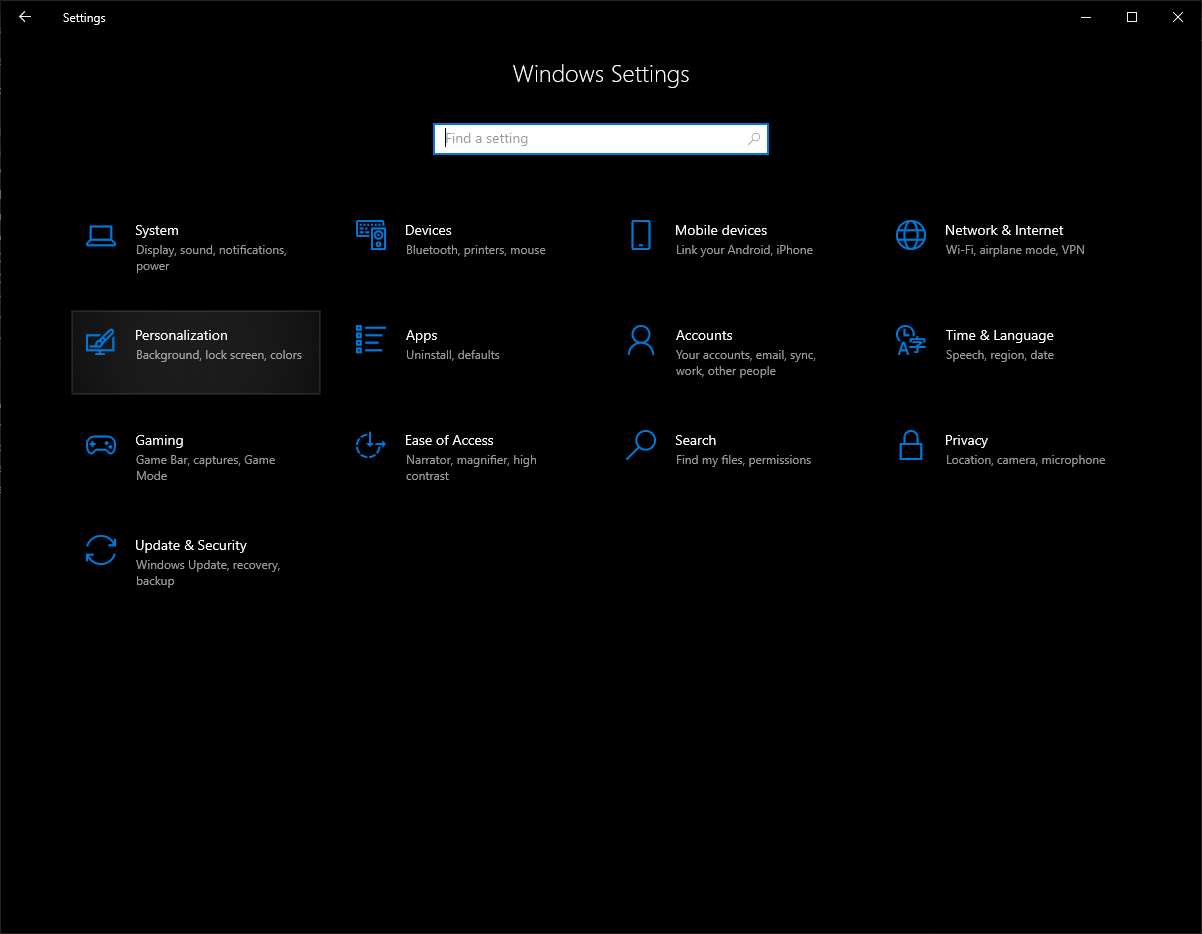
\includegraphics[width=0.85\linewidth, height=0.5\textheight,keepaspectratio]{Imagenes/fe_dark_mode01}
	\caption{Settings\textrightarrow Personalization}
	\label{fig:fedarkmode01}
\end{figure}

\begin{figure}[H]
	\centering
	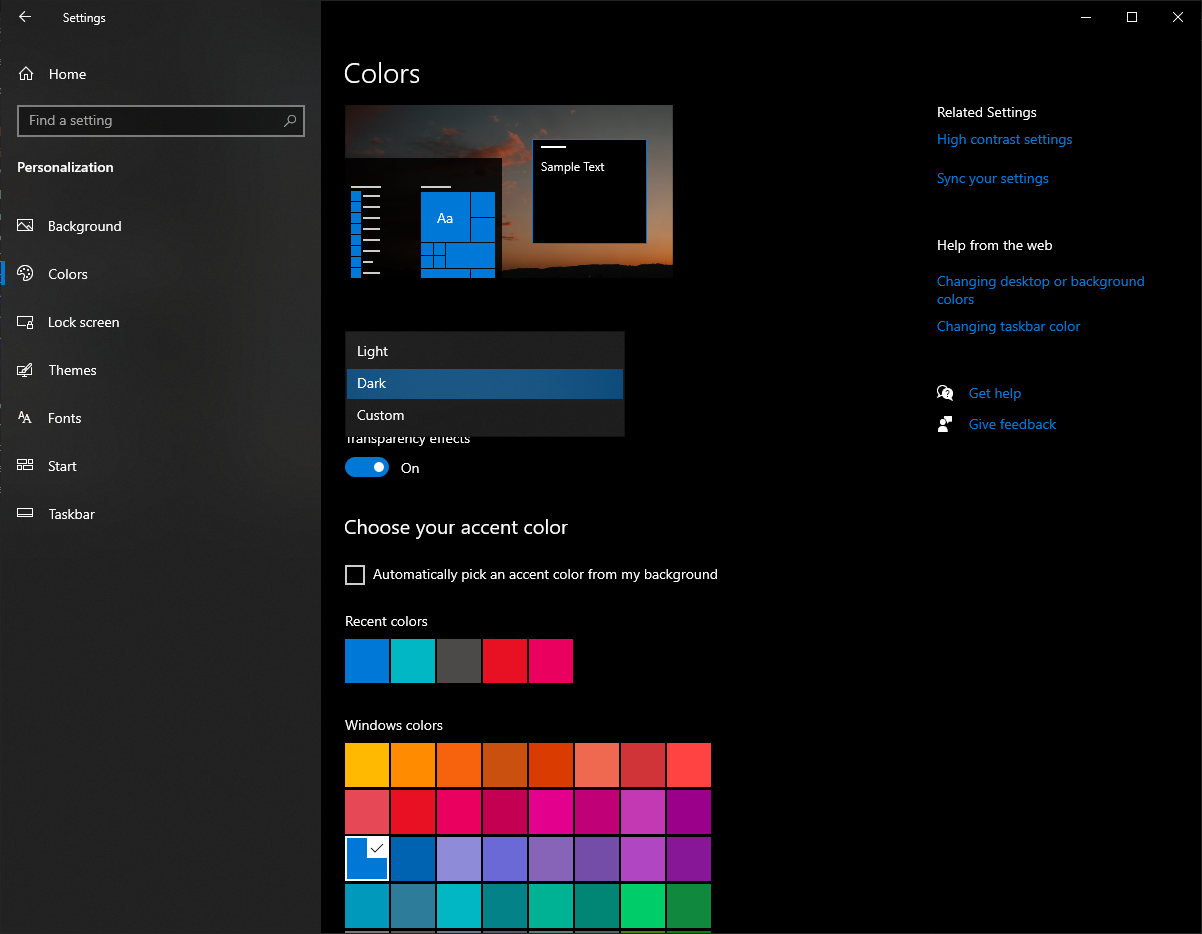
\includegraphics[width=0.85\linewidth, height=0.5\textheight,keepaspectratio]{Imagenes/fe_dark_mode02}
	\caption{Colors\textrightarrow Dark}
	\label{fig:fedarkmode02}
\end{figure}

\begin{figure}[H]
	\centering
	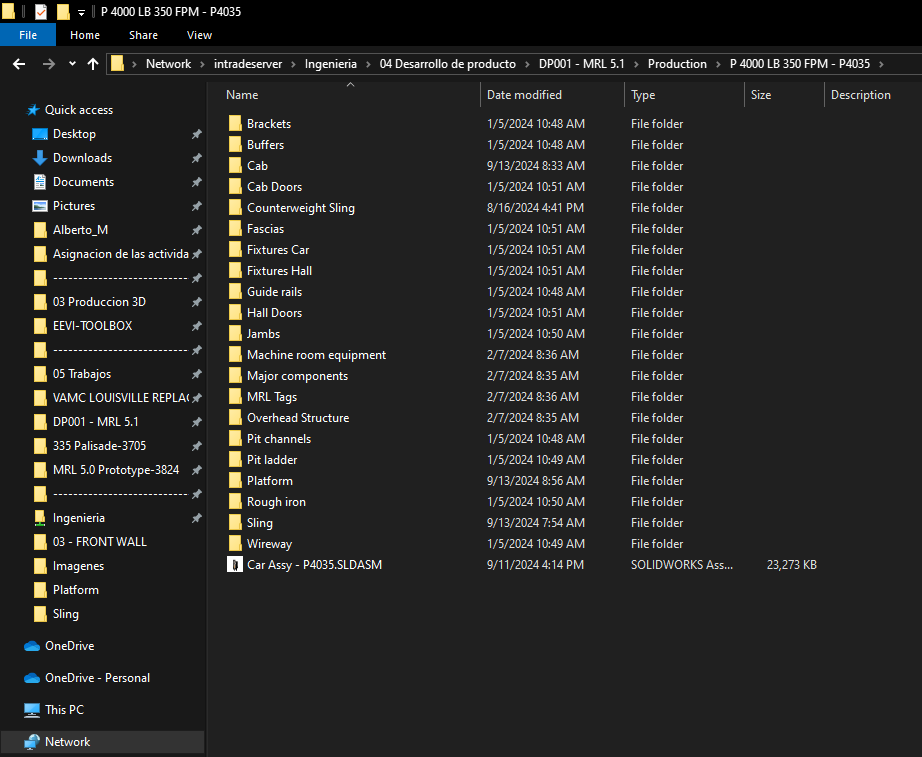
\includegraphics[width=0.85\linewidth, height=0.5\textheight,keepaspectratio]{Imagenes/fe_dark_mode03}
	\caption{Muestra del modo obscuro en el File Explorer}
	\label{fig:fedarkmode03}
\end{figure}


\chapter{Property Description}
	
Se pueden agregar las descripciones de los archivos de SolidWorks en el explorador de archivos para una fácil visualización.

\begin{figure}[H]
	\centering
	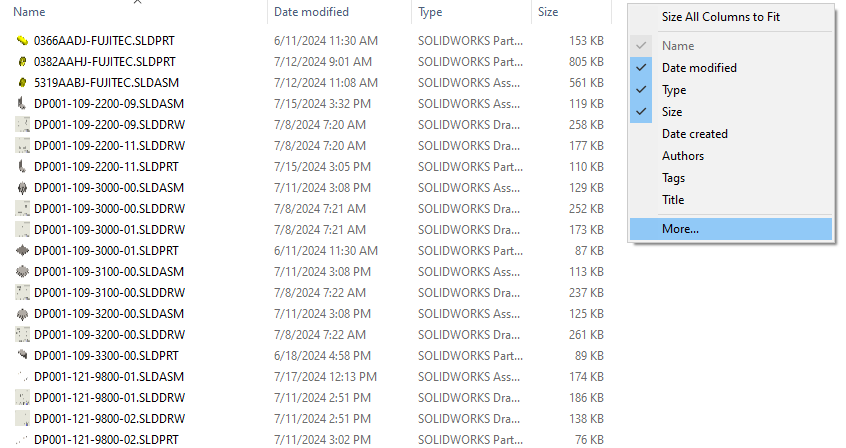
\includegraphics[width=0.95\linewidth, height=0.5\textheight,keepaspectratio]{Imagenes/fe_prop_desc}
	\caption{Click-derecho\textrightarrow More}
	\label{fig:fepropdesc}
\end{figure}

\begin{figure}[H]
	\centering
	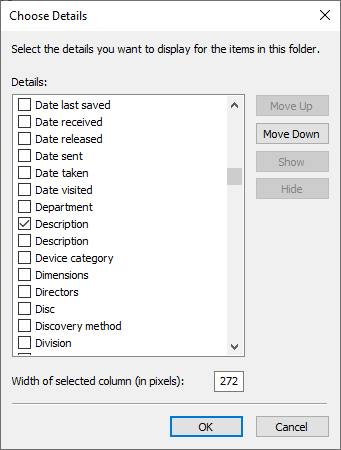
\includegraphics[width=0.65\linewidth, height=0.5\textheight,keepaspectratio]{Imagenes/fe_prop_desc_02}
	\caption{Seleccionar el 2\textsuperscript{do} \emph{Description}\textrightarrow OK}
	\label{fig:fepropdesc02}
\end{figure}

\begin{figure}[H]
	\centering
	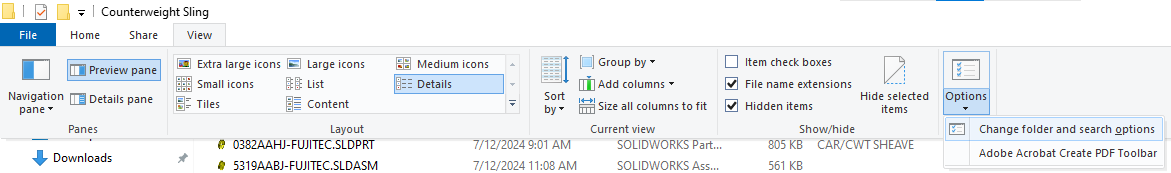
\includegraphics[width=0.95\linewidth, height=0.5\textheight,keepaspectratio]{Imagenes/fe_prop_desc_03}
	\caption{View\textrightarrow Options Change\textrightarrow Folder and search options}
	\label{fig:fepropdesc03}
\end{figure}

\begin{figure}[H]
	\centering
	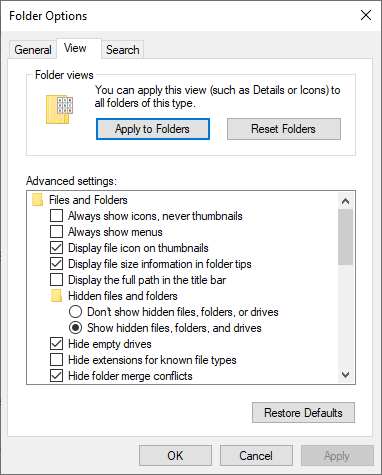
\includegraphics[width=0.85\linewidth, height=0.5\textheight,keepaspectratio]{Imagenes/fe_prop_desc_04}
	\caption{View\textrightarrow Apply to Folders}
	\label{fig:fepropdesc04}
\end{figure}

\begin{figure}[H]
	\centering
	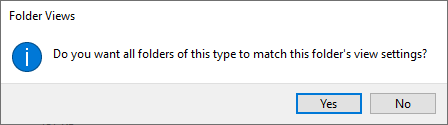
\includegraphics[width=0.85\linewidth, height=0.5\textheight,keepaspectratio]{Imagenes/fe_prop_desc_05}
	\caption{Seleccionar Yes}
	\label{fig:fepropdesc05}
\end{figure}

\clearpage

{\LARGE Resultado}

\begin{figure}[H]
	\centering
	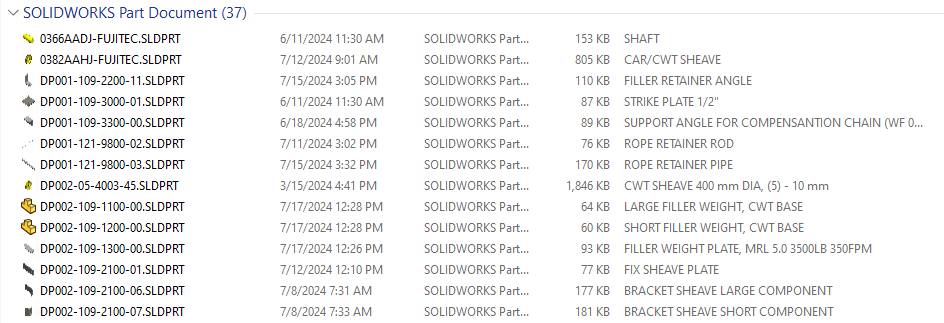
\includegraphics[width=0.95\linewidth, height=0.5\textheight,keepaspectratio]{Imagenes/fe_prop_desc_06}
	\caption{Resultado del property description}
	\label{fig:fepropdesc06}
\end{figure}

\chapter{División en el sidebar}

Se puede dividir el sidebar para tener una organización de las carpetas en acceso rápido.

\begin{figure}[H]
	\centering
	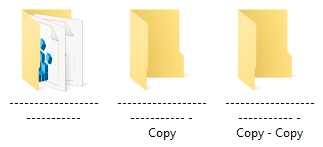
\includegraphics[width=0.55\linewidth,height=0.45\textheight,keepaspectratio]{Imagenes/fe_division_01}
	\caption{Crear carpetas con el nombre `` --------- "}
	\label{fig:fedivision01}
\end{figure}

\begin{figure}[H]
	\centering
	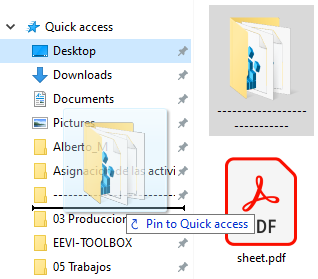
\includegraphics[width=0.55\linewidth, height=0.45\textheight,keepaspectratio]{Imagenes/fe_division_02}
	\caption{Fijarlas en el sidebar}
	\label{fig:fedivision02}
\end{figure}

\clearpage

{\LARGE Resultado}

\begin{figure}[H]
	\centering
	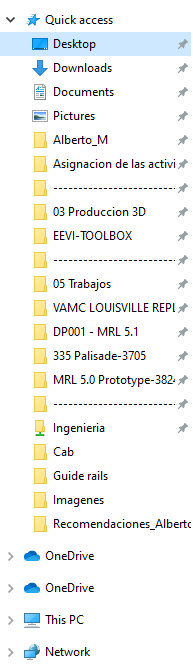
\includegraphics[width=0.75\linewidth, height=0.75\textheight,keepaspectratio]{Imagenes/fe_division_03}
	\caption{Resultado de la división en el sidebar}
	\label{fig:fedivision03}
\end{figure}

\part{Outlook}

\chapter{Create Folders}

Se pueden crear carpetas para organizar la bandeja de entrada.

\begin{figure}[H]
	\centering
	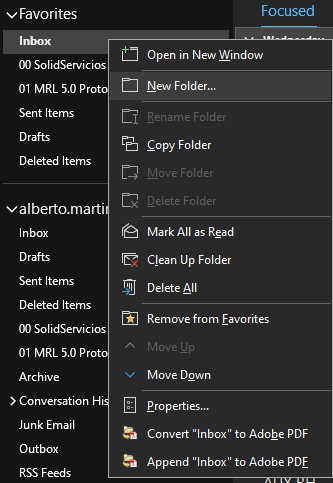
\includegraphics[width=0.85\linewidth, height=0.5\textheight,keepaspectratio]{Imagenes/outlook_createfolders01}
	\caption{Click-derecho y seleccionar \emph{New Folder}}
	\label{fig:outlookcreatefolders01}
\end{figure}

\begin{figure}[H]
	\centering
	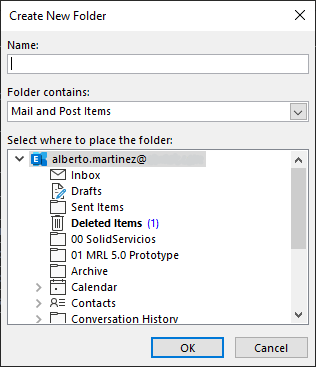
\includegraphics[width=0.65\linewidth, height=0.45\textheight,keepaspectratio]{Imagenes/outlook_createfolders02}
	\caption{Introducir el nombre de la carpeta}
	\label{fig:outlookcreatefolders02}
\end{figure}

{\LARGE Resultado}

\begin{figure}[H]
	\centering
	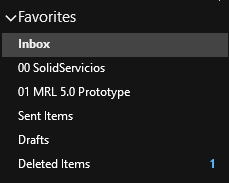
\includegraphics[width=0.55\linewidth, height=0.35\textheight,keepaspectratio]{Imagenes/outlook_createfolders03}
	\caption{Carpetas en el inbox}
	\label{fig:outlookcreatefolders03}
\end{figure}

\chapter{Find Related Messages}

Al hacer click-derecho sobre un correo se puede seleccionar la función \emph{Find Related} que sirve para facilitar buscar correos.

Es util cuando se están organizando los correos en carpetas por primera vez.

\begin{figure}[H]
	\centering
	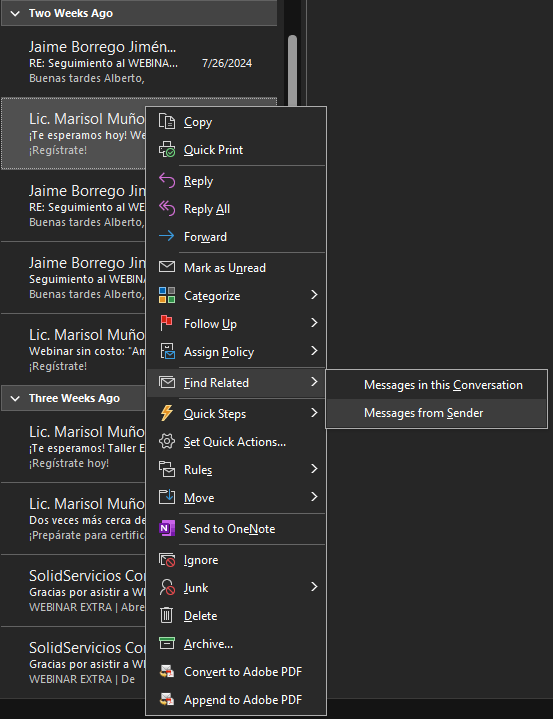
\includegraphics[width=0.85\linewidth, height=0.5\textheight,keepaspectratio]{Imagenes/outlook_findrelated01}
	\caption{Seleccionar el modo de busqueda que se desee}
	\label{fig:outlookfindrelated01}
\end{figure}

\vskip50pt

{\LARGE Resultado}

\begin{figure}[H]
	\centering
	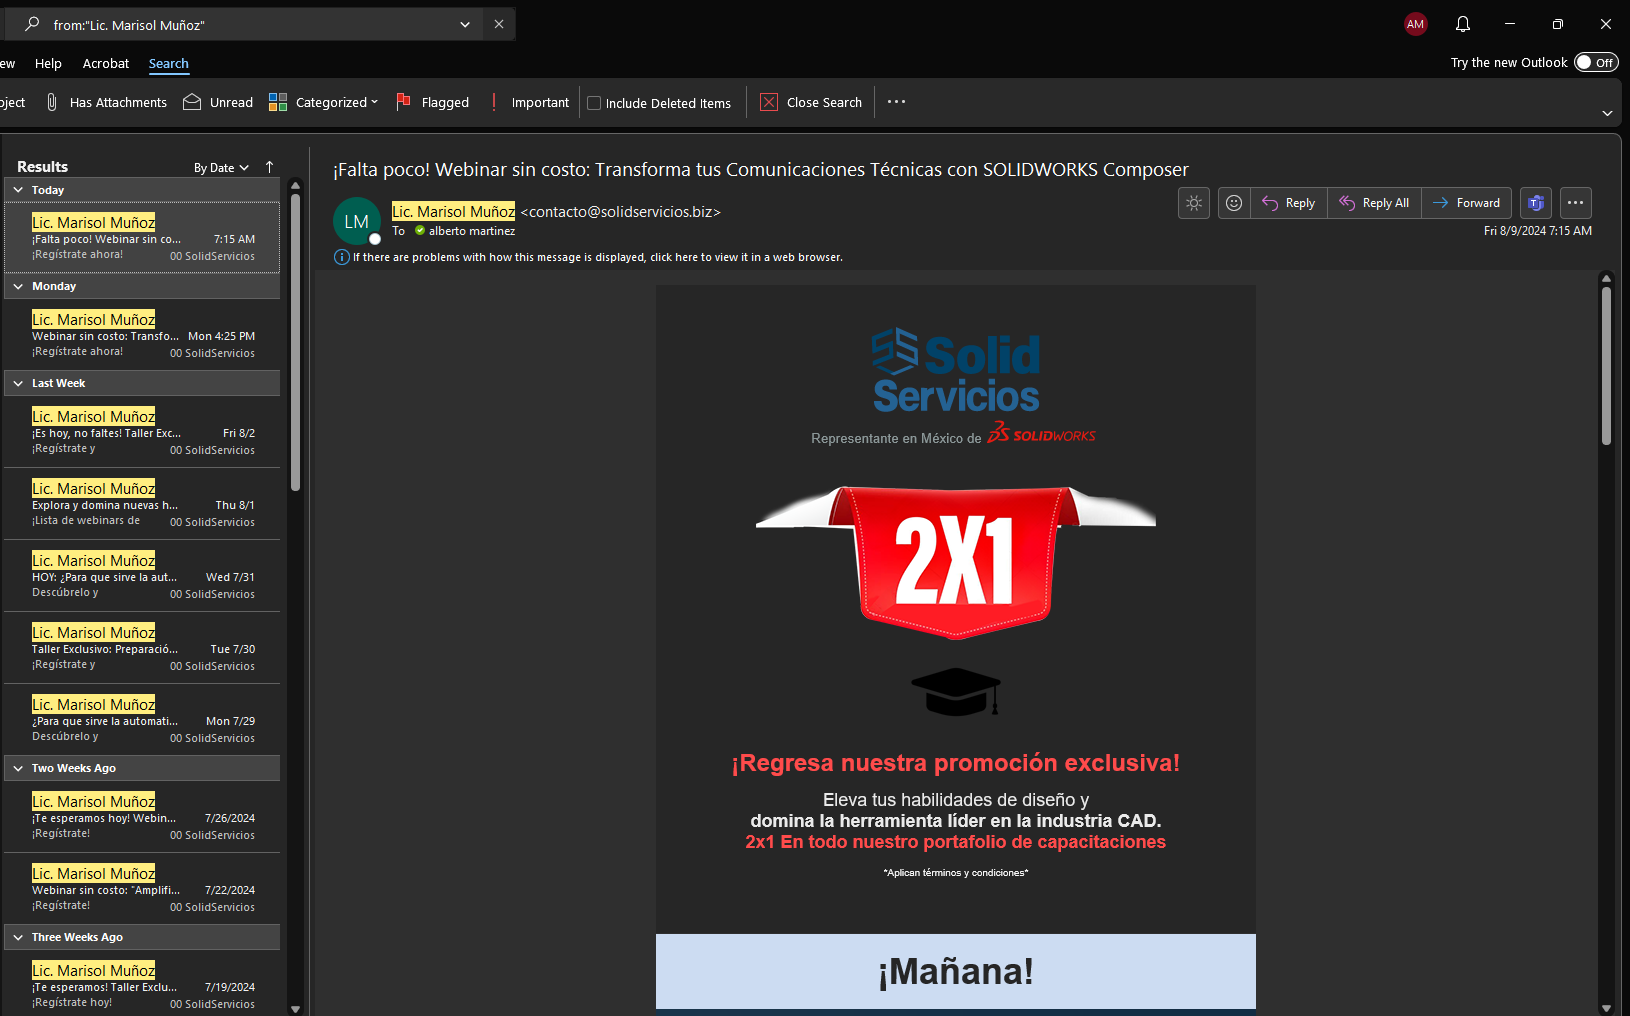
\includegraphics[width=0.95\linewidth, height=0.55\textheight,keepaspectratio]{Imagenes/outlook_findrelated02}
	\caption{Busqueda por \emph{Messages From Sender}}
	\label{fig:outlookfindrelated02}
\end{figure}

\chapter{Rules}

Se pueden crear reglas para mover correos a carpetas automaticamente cuando se reciben. Se accesan al hacer click-derecho bajo la opción de \emph{Rules}.

\section{Always Move Messages From: Sender}

\begin{figure}[H]
	\centering
	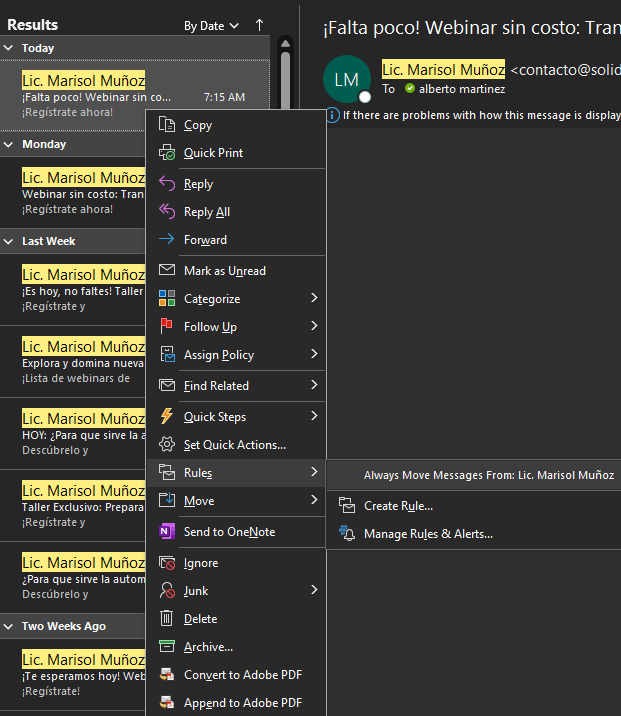
\includegraphics[width=0.85\linewidth, height=0.45\textheight,keepaspectratio]{Imagenes/outlook_rules01}
	\caption{Se selecciona la opción}
	\label{fig:outlookrules01}
\end{figure}

\begin{figure}[H]
	\centering
	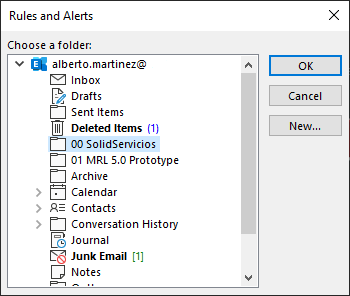
\includegraphics[width=0.75\linewidth, height=0.35\textheight,keepaspectratio]{Imagenes/outlook_rules02}
	\caption{Se selecciona la carpeta a donde se moverán}
	\label{fig:outlookrules02}
\end{figure}

\section{Create Rule}


\begin{figure}[H]
	\centering
	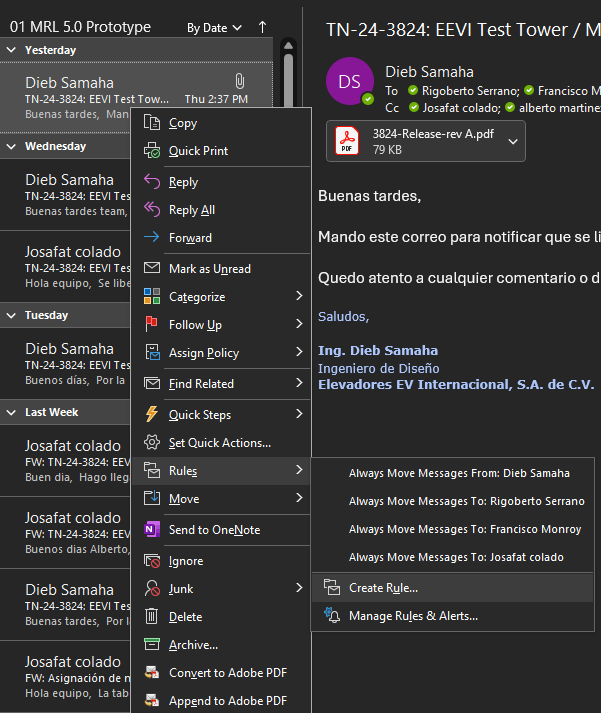
\includegraphics[width=0.75\linewidth, height=0.35\textheight,keepaspectratio]{Imagenes/outlook_rules03}
	\caption{Se selecciona la opción}
	\label{fig:outlookrules03}
\end{figure}

\begin{figure}[H]
	\centering
	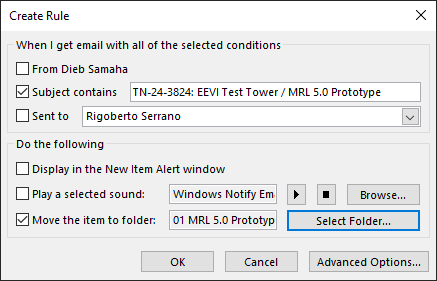
\includegraphics[width=0.75\linewidth, height=0.35\textheight,keepaspectratio]{Imagenes/outlook_rules04}
	\caption{Se seleccionan las opciones de la regla}
	\label{fig:outlookrules04}
\end{figure}

Es posible ejecutar la regla en la carpeta actual y mover los correos que ya se habían recibido anteriormente.

\begin{figure}[H]
	\centering
	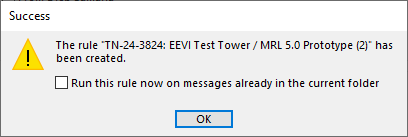
\includegraphics[width=0.75\linewidth, height=0.35\textheight,keepaspectratio]{Imagenes/outlook_rules05}
	\caption{Aplicar la regla a la carpeta acutal}
	\label{fig:outlookrules05}
\end{figure}

\section{Edit Rules}

Se pueden editar o visualizar las reglas creadas previamente.

\begin{figure}[H]
	\centering
	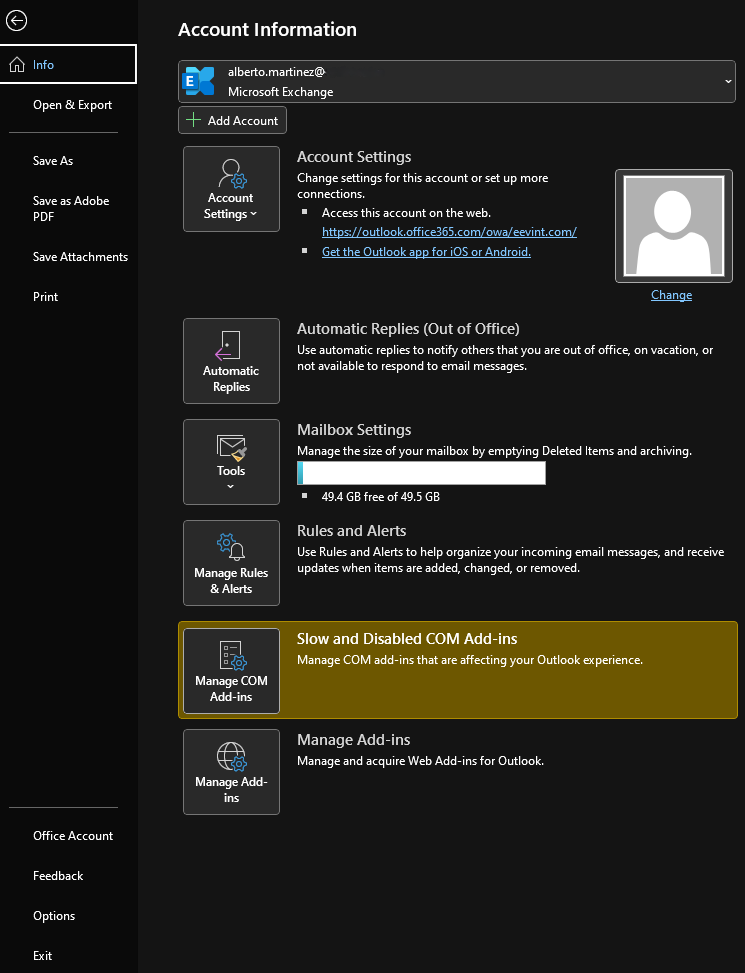
\includegraphics[width=0.75\linewidth, height=0.45\textheight,keepaspectratio]{Imagenes/outlook_rules06}
	\caption{File\textrightarrow Rules and Alerts}
	\label{fig:outlookrules06}
\end{figure}

\begin{figure}[H]
	\centering
	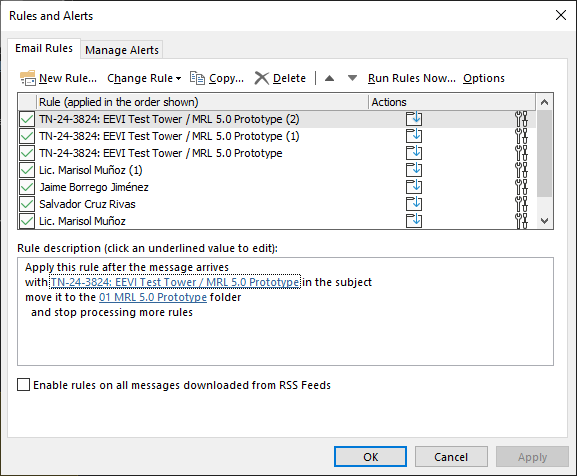
\includegraphics[width=0.75\linewidth, height=0.35\textheight,keepaspectratio]{Imagenes/outlook_rules07}
	\caption{Manejar las reglas}
	\label{fig:outlookrules07}
\end{figure}


\part{AutoCAD}

\chapter{Display Resolution}

Se incrementa la resolución de los círculos y arcos para tener una mayor fidelidad de imagen.

\begin{figure}[H]
	\centering
	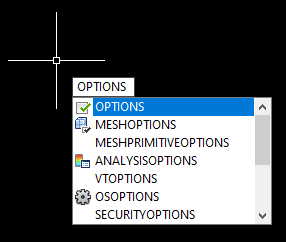
\includegraphics[width=0.75\linewidth, height=0.5\textheight,keepaspectratio]{Imagenes/autocad_display_resolution_01}
	\caption{Options\textrightarrow Display}
	\label{fig:autocaddisplayresolution01}
\end{figure}

\begin{figure}[H]
	\centering
	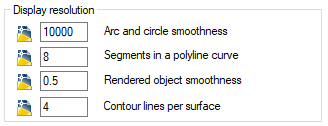
\includegraphics[width=0.85\linewidth, height=0.5\textheight,keepaspectratio]{Imagenes/autocad_display_resolution_02}
	\caption{Cambiar display resolution a los siguientes valores}
	\label{fig:autocaddisplayresolution02}
\end{figure}
%reemplazar esta foto por una donde salgan los dos

{\LARGE Resultado}

\begin{figure}[H]
	\centering
	\begin{subfigure}[b]{0.45\textwidth}
		
\includegraphics[width=\textwidth]{Imagenes/autocad_display_resolution_03}
		\caption{Antes}
		\label{fig:autocaddisplayresolution03}
	\end{subfigure}
		\begin{subfigure}[b]{0.45\textwidth}
		
\includegraphics[width=\textwidth]{Imagenes/autocad_display_resolution_04}
		\caption{Después}
		\label{fig:autocaddisplayresolution04}
	\end{subfigure}
	\caption{Resultado de display resolution}
\end{figure}

\chapter{Modelspace y Paperspace Background}

Se puede configurar el fondo del programa a cualquier color que se desee.

\begin{figure}[H]
	\centering
	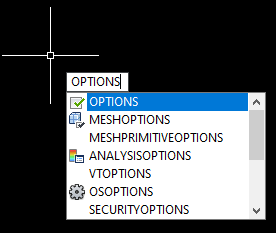
\includegraphics[width=0.75\linewidth, height=0.5\textheight,keepaspectratio]{Imagenes/autocad_background_01}
	\caption{Options\textrightarrow Display}
	\label{fig:autocadbackground01}
\end{figure}

\begin{figure}[H]
	\centering
	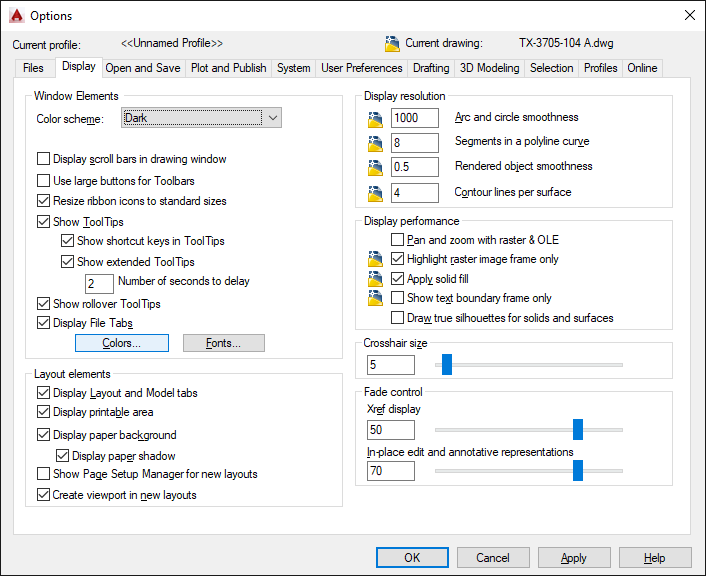
\includegraphics[width=0.75\linewidth, height=0.5\textheight,keepaspectratio]{Imagenes/autocad_background_02}
	\caption{Window Elements\textrightarrow Colors}
	\label{fig:autocadbackground02}
\end{figure}

\begin{figure}[H]
	\centering
	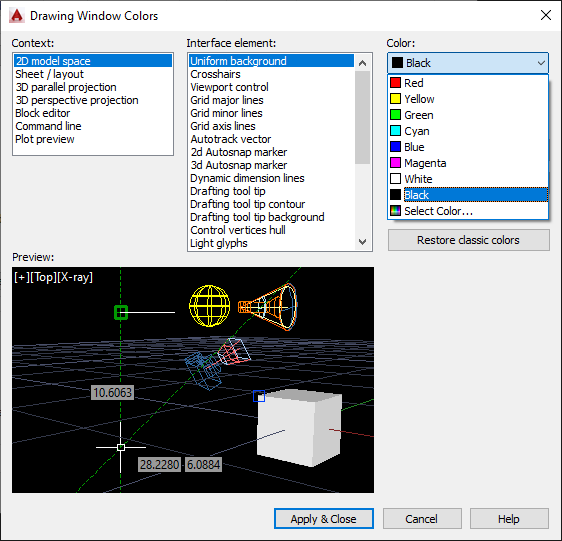
\includegraphics[width=0.75\linewidth, height=0.5\textheight,keepaspectratio]{Imagenes/autocad_background_03}
	\caption{2D Model Space\textrightarrow Uniform Background\textrightarrow Color}
	\label{fig:autocadbackground03}
\end{figure}

\clearpage

{\LARGE Resultado}

\begin{figure}[H]
	\centering
	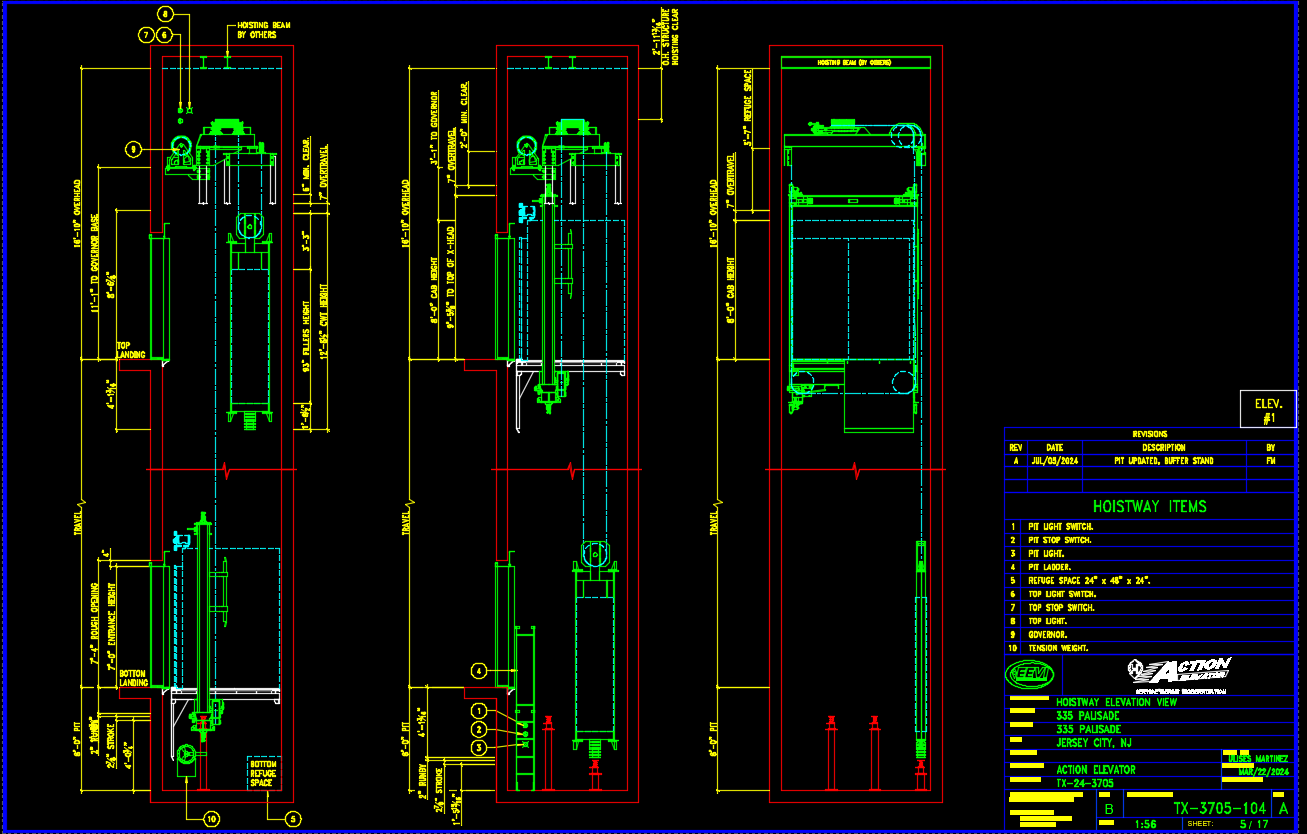
\includegraphics[width=0.65\linewidth, height=0.5\textheight,keepaspectratio]{Imagenes/autocad_background_04}
	\caption{Resultado del modelspace y paperspace background}
	\label{fig:autocadbackground04}
\end{figure}

\chapter{Confirm Commands}

Usar \emph{Spacebar} para confirmar comandos. \textbf{NO} usar Enter.

Se recomienda que todos los comandos sean ejecutados el la ventana de comandos y no buscando el ícono en el ribbon.

\begin{figure}[H]
	\centering
	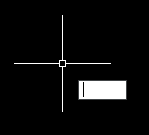
\includegraphics[width=0.65\linewidth, height=0.5\textheight,keepaspectratio]{Imagenes/autocad_spacebar01}
	\caption{Ventana para introducir comandos}
	\label{fig:autocadspacebar01}
\end{figure}


\chapter{Publish Multiple PDF}

Se pueden crear archivos PDF de múltiples dibujos al mismo tiempo utilizando el comando \emph{Publish}.

\begin{figure}[H]
	\centering
	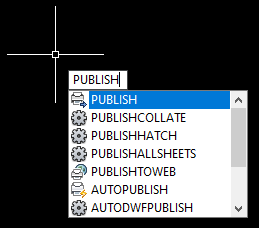
\includegraphics[width=0.75\linewidth, height=0.5\textheight,keepaspectratio]{Imagenes/autocad_publish_01}
	\caption{Publish}
	\label{fig:autocadpublish01}
\end{figure}

\begin{figure}[H]
	\centering
	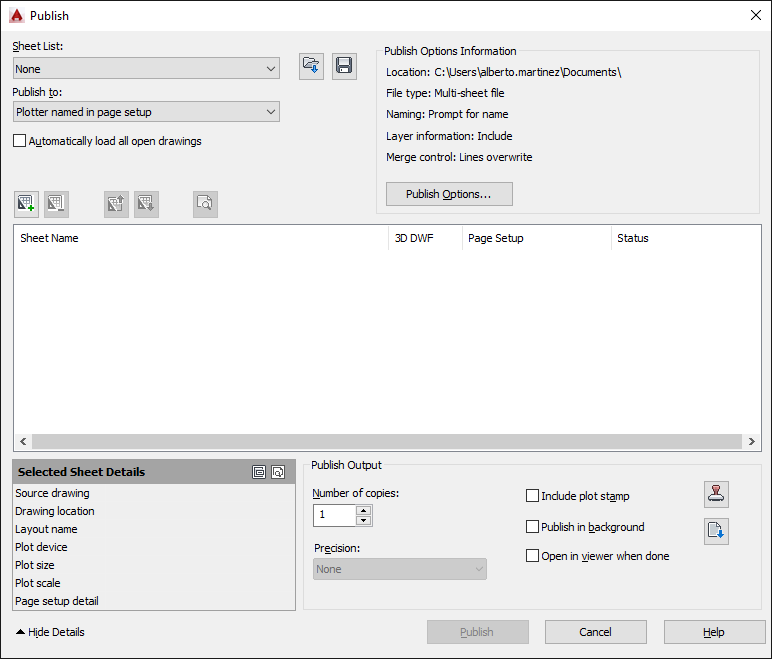
\includegraphics[width=0.85\linewidth, height=0.5\textheight,keepaspectratio]{Imagenes/autocad_publish_02}
	\caption{Borrar la hoja predeterminada}
	\label{fig:autocadpublish02}
\end{figure}

\begin{figure}[H]
	\centering
	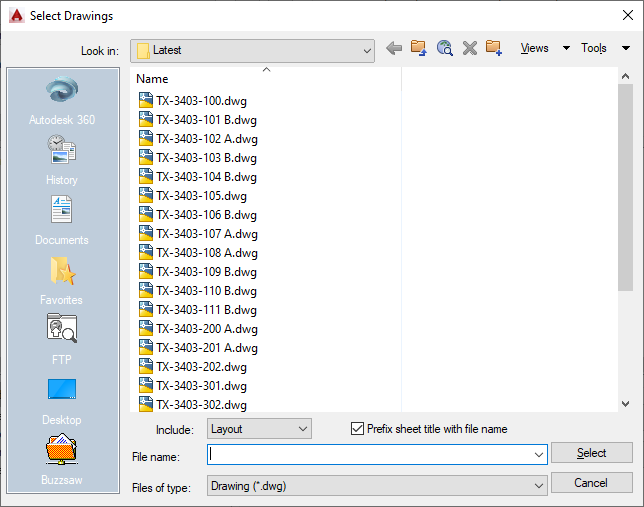
\includegraphics[width=0.85\linewidth, height=0.5\textheight,keepaspectratio]{Imagenes/autocad_publish_03}
	\caption{Add Sheets\textrightarrow Seleccionar los dibujos que se quieren imprimir}
	\label{fig:autocadpublish03}
\end{figure}


\begin{center}
	\fbox{SELECCIONAR LAYOUT ONLY}
\end{center}



{\LARGE Resultado}

\begin{figure}[H]
	\centering
	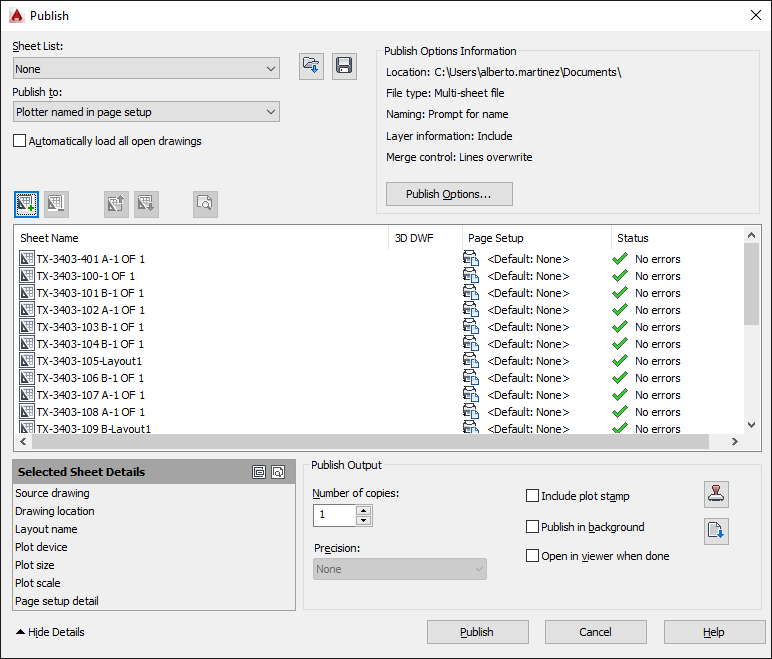
\includegraphics[width=0.85\linewidth, height=0.5\textheight,keepaspectratio]{Imagenes/autocad_publish_04}
	\caption{Resultado de seleccionar multiples layouts para imprimir}
	\label{fig:autocadpublish04}
\end{figure}


\chapter{Ray}

Con el comando \emph{Ray} se define un primer punto que será el origen de la linea infinitamente larga y luego un segundo punto que marca la dirección. Es util para hacer proyecciones.

\begin{figure}[H]
	\centering
	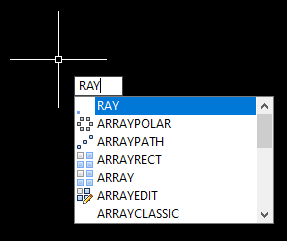
\includegraphics[width=0.65\linewidth, height=0.5\textheight,keepaspectratio]{Imagenes/autocad_ray01}
	\caption{Ray}
	\label{fig:autocadray01}
\end{figure}

\begin{figure}[H]
	\centering
	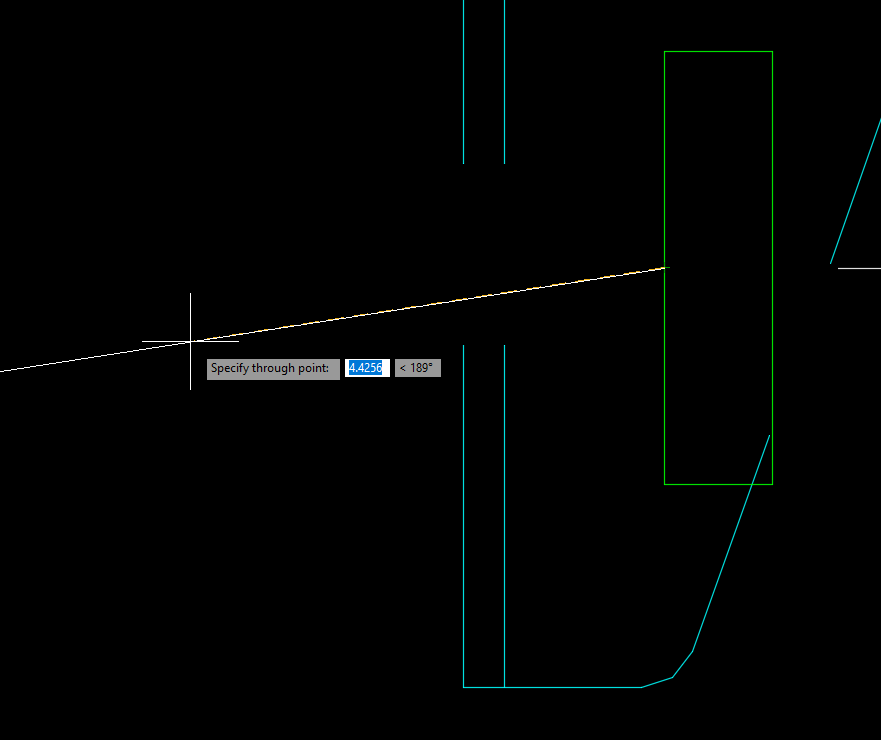
\includegraphics[width=0.75\linewidth, height=0.5\textheight,keepaspectratio]{Imagenes/autocad_ray02}
	\caption{Una vez definido el primer punto como origen se selecciona otro como la dirección}
	\label{fig:autocadray02}
\end{figure}

\begin{figure}[H]
	\centering
	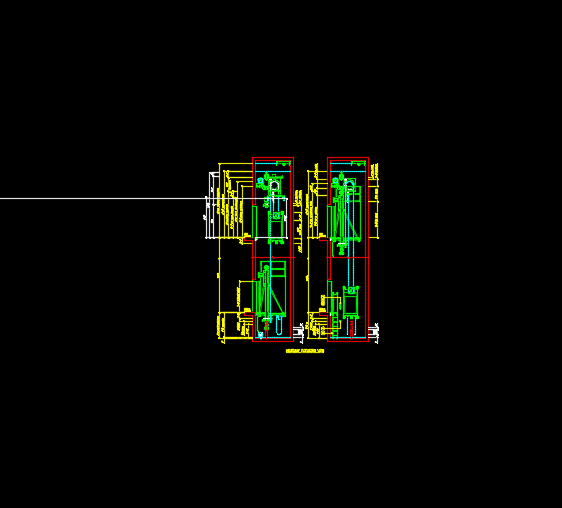
\includegraphics[width=0.85\linewidth, height=0.5\textheight,keepaspectratio]{Imagenes/autocad_ray03}
	\caption{La linea creada tiene una longitud infinitamente larga}
	\label{fig:autocadray03}
\end{figure}

\begin{figure}[H]
	\centering
	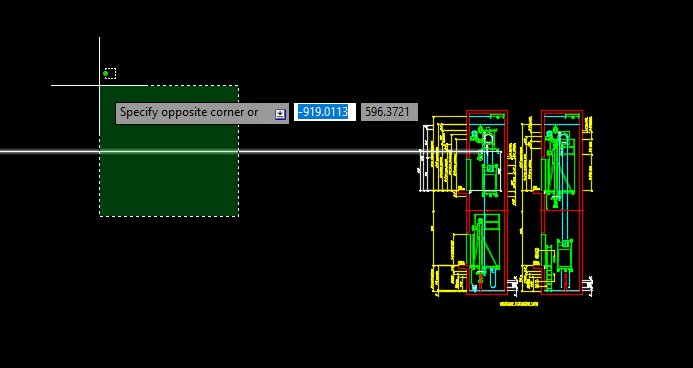
\includegraphics[width=0.85\linewidth, height=0.5\textheight,keepaspectratio]{Imagenes/autocad_ray04}
	\caption{La linea puede ser borrada facilmente}
	\label{fig:autocadray04}
\end{figure}



\chapter{Stretch}

Con el comando \emph{Stretch} se pueden modificar los nodos de los elementos moviendolos de posición.

\begin{figure}[H]
	\centering
	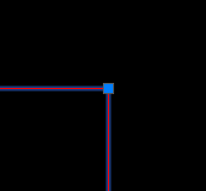
\includegraphics[width=0.85\linewidth, height=0.5\textheight,keepaspectratio]{Imagenes/autocad_stretch01}
	\caption{Un nodo}
	\label{fig:autocadstretch01}
\end{figure}

\begin{figure}[H]
	\centering
	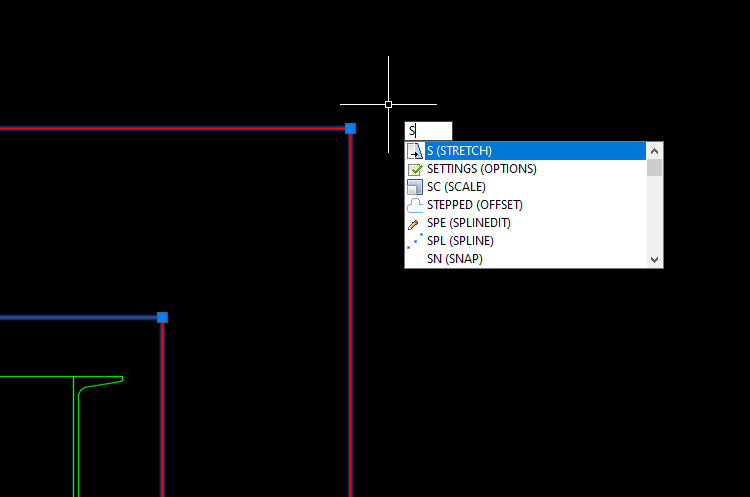
\includegraphics[width=0.85\linewidth, height=0.5\textheight,keepaspectratio]{Imagenes/autocad_stretch02}
	\caption{Stretch}
	\label{fig:autocadstretch02}
\end{figure}

\begin{figure}[H]
	\centering
	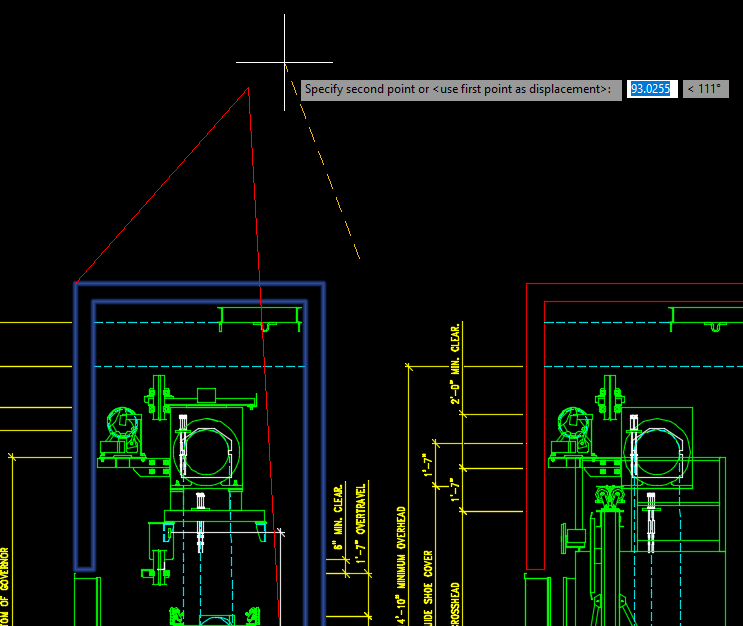
\includegraphics[width=0.85\linewidth, height=0.5\textheight,keepaspectratio]{Imagenes/autocad_stretch03}
	\caption{Se pueden cambiar la posición de los nodos}
	\label{fig:autocadstretch03}
\end{figure}


\chapter{Create Alias}

Se pueden reconfigurar los atajos para llamar un comando.

\begin{figure}[H]
	\centering
	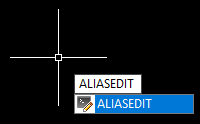
\includegraphics[width=0.65\linewidth, height=0.5\textheight,keepaspectratio]{Imagenes/autocad_alias_01}
	\caption{Aliasedit}
	\label{fig:autocadalias01}
\end{figure}

\begin{figure}[H]
	\centering
	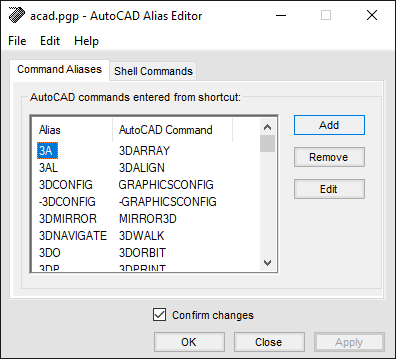
\includegraphics[width=0.75\linewidth, height=0.5\textheight,keepaspectratio]{Imagenes/autocad_alias_02}
	\caption{Seleccionar Add}
	\label{fig:autocadalias02}
\end{figure}

\section{Publish}

\begin{figure}[H]
	\centering
	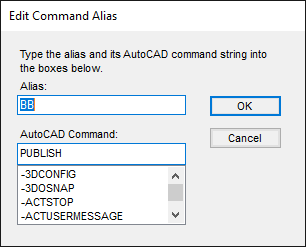
\includegraphics[width=0.75\linewidth, height=0.5\textheight,keepaspectratio]{Imagenes/autocad_alias_publish_01}
	\caption{Command Alias para Publish}
	\label{fig:autocadaliaspublish01}
\end{figure}

\begin{figure}[H]
	\centering
	\begin{subfigure}[b]{0.43\textwidth}
		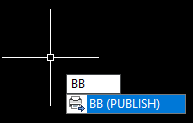
\includegraphics[width=\textwidth]{Imagenes/autocad_alias_publish_02}
		\caption{Teclear el alias}
		\label{fig:autocadaliaspublish02}
	\end{subfigure}
	\begin{subfigure}[b]{0.45\textwidth}
		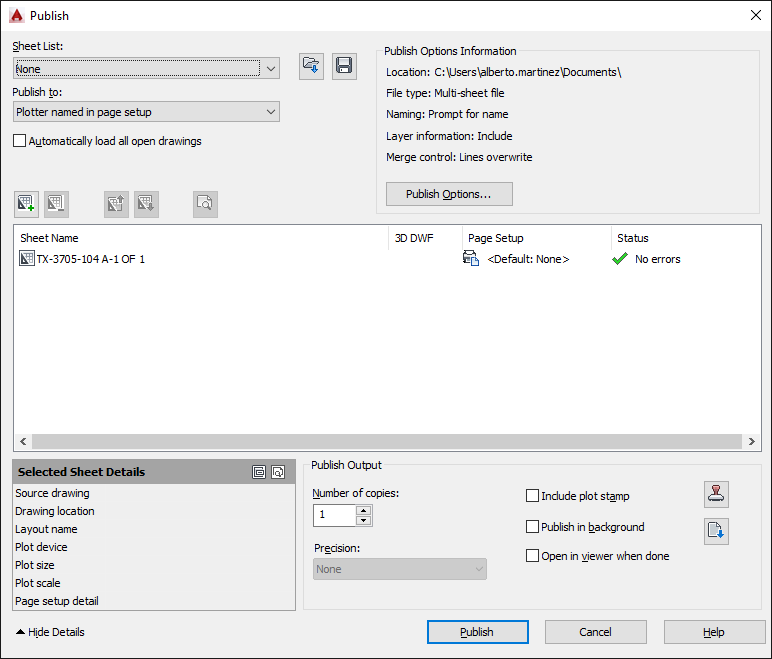
\includegraphics[width=\textwidth]{Imagenes/autocad_alias_publish_03}
		\caption{Ejecuta el comando publish}
		\label{fig:autocadaliaspublish03}
	\end{subfigure}
	\caption{Resultado del alias para Publish}
\end{figure}



\section{Quit Modelspace}

Para ser usado cuando se quiere salir del modelspace dentro de la hoja de layout.

\begin{figure}[H]
	\centering
	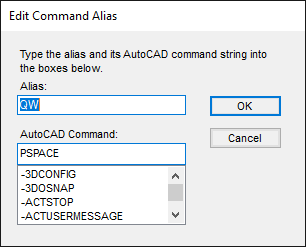
\includegraphics[width=0.7\linewidth, height=0.45\textheight,keepaspectratio]{Imagenes/autocad_alias_quitmodelspace}
	\caption{Command Alias para Paperspace}
	\label{fig:autocadaliasquitmodelspace}
\end{figure}

\section{Ray}

Para ser usado cuando se quiere crear un rayo.

\begin{figure}[H]
	\centering
	\includegraphics[width=0.7\linewidth, height=0.45\textheight,keepaspectratio]{Imagenes/autocad_alias_ray}
	\caption{Command Alias para Ray}
	\label{fig:autocadaliasray}
\end{figure}

\section{Linear Dimension}

Para ser usado cuando se quiere crear una cota linear.

\begin{figure}[H]
	\centering
	\includegraphics[width=0.7\linewidth, height=0.45\textheight,keepaspectratio]{Imagenes/autocad_alias_lineardimension}
	\caption{Command Alias para Dimension Linear}
	\label{fig:autocadaliaslineardimension}
\end{figure}



\section{Layer Options}

\subsection{Esconder el layer seleccionado}

\begin{figure}[H]
	\centering
	\includegraphics[width=0.7\linewidth, height=0.45\textheight,keepaspectratio]{Imagenes/autocad_alias_layeroptions_01}
	\caption{Command Alias para Layer Off}
	\label{fig:autocadaliaslayeroptions01}
\end{figure}

\subsection{Encender todos los layers}

\begin{figure}[H]
	\centering
	\includegraphics[width=0.7\linewidth, height=0.45\textheight,keepaspectratio]{Imagenes/autocad_alias_layeroptions_02}
	\caption{Commnand Alias para Layer On}
\end{figure}

\subsection{Mostrar solo el layer seleccionado}

\begin{figure}[H]
	\centering
	\includegraphics[width=0.7\linewidth, height=0.45\textheight,keepaspectratio]{Imagenes/autocad_alias_layeroptions_03}
	\caption{Command Alias para Layer Isolate}
	\label{fig:autocadaliaslayeroptions03}
\end{figure}

\subsection{Congelar el layer seleccionado}

\begin{figure}[H]
	\centering
	\includegraphics[width=0.75\linewidth, height=0.45\textheight,keepaspectratio]{Imagenes/autocad_alias_layeroptions_04}
	\caption{Command Alias para Layer Freeze}
	\label{fig:autocadaliaslayeroptions04}
\end{figure}


\chapter{Measure Geometry}

\begin{figure}[H]
	\centering
	\includegraphics[width=0.55\linewidth, height=0.35\textheight,keepaspectratio]{Imagenes/autocad_measuregeom01}
	\caption{Manage \textrightarrow Record}
	\label{fig:autocadmeasuregeom01}
\end{figure}

\begin{figure}[H]
	\centering
	\includegraphics[width=0.65\linewidth, height=0.35\textheight,keepaspectratio]{Imagenes/autocad_measuregeom02}
	\caption{MEASUREGEOM + D \textrightarrow Stop}
	\label{fig:autocadmeasuregeom02}
\end{figure}

\begin{figure}[H]
	\centering
	\includegraphics[width=0.75\linewidth, height=0.45\textheight,keepaspectratio]{Imagenes/autocad_measuregeom03}
	\caption{Nombrar el macro \emph{D}}
	\label{fig:autocadmeasuregeom03}
\end{figure}

\begin{figure}[H]
	\centering
	\includegraphics[width=0.95\linewidth, height=0.5\textheight,keepaspectratio]{Imagenes/autocad_measuregeom04}
	\caption{Al escribir \emph{D} se ejecuta la acción}
	\label{fig:autocadmeasuregeom04}
\end{figure}

\begin{figure}[H]
	\centering
	\includegraphics[width=0.95\linewidth, height=0.5\textheight,keepaspectratio]{Imagenes/autocad_measuregeom05}
	\caption{Acción ejecutada}
	\label{fig:autocadmeasuregeom05}
\end{figure}


\chapter{Right-Click Selection Options}

Al oprimir \emph{CTRL + Click-derecho} se despliega un menú donde se puede elegir un punto de referencia con el comando \emph{From}, el punto medio entre dos puntos con \emph{Mid Between 2 Points} o restringir el movimiento a uno de los ejes con \emph{Point Filters}.

\begin{figure}[H]
	\centering
	\includegraphics[width=0.85\linewidth, height=0.45\textheight,keepaspectratio]{Imagenes/autocad_rightclickmenu01}
	\caption{Menú de opciones}
	\label{fig:autocadrightclickmenu01}
\end{figure}













\part{SolidWorks}

\chapter{Dark Mode}

Se puede cambiar el color de la interfaz y el color de los diferentes elementos dentro de SolidWorks.

\begin{figure}[H]
	\centering
	\includegraphics[width=0.95\linewidth, height=0.65\textheight,keepaspectratio]{Imagenes/solidworks_dark_mode01}
	\caption{System Options\textrightarrow Colors}
	\label{fig:solidworksdarkmode01}
\end{figure}

\begin{itemize}
	\item Dentro de \emph{Background} se puede cambiar a \emph{Dark} para un modo obscuro
	\item En color scheme puedes seleccionar los colores de diferentes elementos
	\item En \emph{Background appearance} se puede cambiar el fondo del área gráfica
\end{itemize}

\begin{figure}[H]
	\centering
	\includegraphics[width=0.95\linewidth, height=0.75\textheight,keepaspectratio]{Imagenes/solidworks_dark_mode02}
	\caption{System Options\textrightarrow Colors}
	\label{fig:solidworksdarkmode02}
\end{figure}


\chapter{Shortcut Bars}

\section{Configuración}

\begin{figure}[H]
	\centering
	\includegraphics[width=0.95\linewidth, height=0.5\textheight,keepaspectratio]{Imagenes/solidworks_shortcutbars_01}
	\caption{Click-derecho\textrightarrow Customize}
	\label{fig:solidworksshortcutbars01}
\end{figure}

\begin{figure}[H]
	\centering
	\includegraphics[width=0.85\linewidth, height=0.5\textheight,keepaspectratio]{Imagenes/solidworks_shortcutbars_02}
	\caption{Shortcut Bars\textrightarrow Arrastrar los siguientes íconos al toolbar}
	\label{fig:solidworksshortcutbars02}
\end{figure}

También es posible agregar comandos en el menú de busqueda superior derecho y en el mismo menú del shortcut (\emph{S}), aunque este no permite agregar los flyouts.

Se recomiendad que la forma de la barra sea la más cuadrada posible y que se coloquen los comandos más frecuentemente usados en la esquina superior izquierda (cerca del cursor) y los menos frecuentes en la esquina inferior derecha (lejos del cursor).

\subsection{Part}

\begin{itemize}
	\item Select Flyout
	\item Extruded Boss/ Base Flyout
	\item Cut Extrude Flyout
	\item Fillet Flyout
	\item Reference Geometry Flyout
	\item Hole Wizard Flyout
	\item Mirror
	\item Linear Pattern Flyout
\end{itemize}

\begin{figure}[H]
	\centering
	\includegraphics[width=0.45\linewidth, height=0.5\textheight,keepaspectratio]{Imagenes/solidworks_shortcutbars_03}
	\caption{Shortcut toolbar para partes}
	\label{fig:solidworksshortcutbars03}
\end{figure}

\subsection{Assembly}

\begin{itemize}
	\item Select Flyout
	\item Mate
	\item Show Hidden Components
	\item Insert Component
	\item Mirror Component
	\item Linear Component Pattern
	\item Edit Component
	\item Replace Components
	\item Reference Geometry Flyout
\end{itemize}

\begin{figure}[H]
	\centering
	\includegraphics[width=0.35\linewidth, height=0.4\textheight,keepaspectratio]{Imagenes/solidworks_shortcutbars_04}
	\caption{Shortcut toolbar para ensambles}
	\label{fig:solidworksshortcutbars04}
\end{figure}

\subsection{Drawing}

\begin{itemize}
	\item Select Flyout
	\item Smart Dimension Flyout
	\item Ordinate Dimension
	\item Drawing Flyout
	\item Hole Callout
	\item Center Mark
	\item Projected View
	\item Balloon
	\item Point
	\item Tables Flyout
	\item Centerline
	\item Annotation Flyout
	\item Sketch Flyout
	\item Replace Model

\end{itemize}

\begin{figure}[H]
	\centering
	\includegraphics[width=0.45\linewidth, height=0.45\textheight,keepaspectratio]{Imagenes/solidworks_shortcutbars_05}
	\caption{Shortcut toolbar para dibujos}
	\label{fig:solidworksshortcutbars05}
\end{figure}

\subsection{Sketch}

\begin{itemize}
	\item Select Flyout
	\item Smart Dimension Flyout
	\item Sketch
	\item Center Rectangle Flyout
	\item Line
	\item Centerline
	\item Circle Flyout
	\item Straight Slot Flyout
	\item Centerpoint Arc Flyout
	\item Sketch Fillet Flyout
	\item Point
	\item Spline Flyout
	\item Trim Entities Flyout
	\item Mirror Entities
	\item Offset Entities
	\item Extruded Boss/ Base Flyout
	\item Cut Extrude Flyout
	\item Base Flange/ Tab
	\item Move Entities
\end{itemize}

\begin{figure}[H]
	\centering
	\includegraphics[width=0.45\linewidth, height=0.5\textheight,keepaspectratio]{Imagenes/solidworks_shortcutbars_06}
	\caption{Shortcut toolbar para sketches}
	\label{fig:solidworksshortcutbars06}
\end{figure}


\section{Uso}

Se despliega el menú de atajo con la tecla \emph{S}.

Se busca que todas las funciones se utilicen con el shortcut bar en vez del ribbon. También tiene una función de búsqueda para funciones en caso de no tenerlas.

Se puede añadir y remover funciones dependiendo del uso personal.

\begin{figure}[H]
	\centering
	\includegraphics[width=0.85\linewidth, height=0.5\textheight,keepaspectratio]{Imagenes/solidworks_shortcutbars_07}
	\caption{El menú se despliega junto al cursor}
	\label{fig:solidworksshortcutbars07}
\end{figure}



\chapter{Comandos del Teclado}

Se pueden reconfigurar los comandos del teclado para tener un acceso más fácil y rapido a ellos.

\begin{figure}[H]
	\centering
	\includegraphics[width=0.85\linewidth, height=0.65\textheight,keepaspectratio]{Imagenes/solidworks_keyboard_01}
	\caption{Customize\textrightarrow Keyboard}
	\label{fig:solidworkskeyboard01}
\end{figure}

\section{Measure}

\begin{figure}[H]
	\centering
	\includegraphics[width=0.85\linewidth, height=0.65\textheight,keepaspectratio]{Imagenes/solidworks_keyboard_02}
	\caption{Buscar el comando y en shortcut usar \emph{Z}}
	\label{fig:solidworkskeyboard02}
\end{figure}

\section{Triad Manipulator}

\begin{figure}[H]
	\centering
	\includegraphics[width=0.85\linewidth, height=0.65\textheight,keepaspectratio]{Imagenes/solidworks_keyboard_03}
	\caption{Buscar el comando y en shortcut usar \emph{C}}
	\label{fig:solidworkskeyboard03}
\end{figure}

\section{Isometric}

\begin{figure}[H]
	\centering
	\includegraphics[width=0.85\linewidth, height=0.65\textheight,keepaspectratio]{Imagenes/solidworks_keyboard_04}
	\caption{Buscar el comando y agregar un shortcut en \emph{CTRL+`}}
	\label{fig:solidworkskeyboard04}
\end{figure}

\chapter{Context Sensitive Left-Click}

Al hacer click-izquierdo en alguna de las dos áreas del programa se despliega un menú de contexto que muestra funciones sugeridas en base a lo que se seleccionó.

\section{Graphics-Area}

\begin{figure}[H]
	\centering
	\includegraphics[width=0.85\linewidth, height=0.5\textheight,keepaspectratio]{Imagenes/solidworks_contextmenu_01}
	\caption{Click-izquierdo dentro del área gráfica\textrightarrow Click-derecho en el menú de contexto\textrightarrow Customize}
	\label{fig:solidworkscontextmenu01}
\end{figure}

Agregar las siguientes funciones:

\begin{itemize}
	\item Mirror
	\item Mirror Entities
	\item Linear Pattern Flyout
	\item Hole Wizard
	\item Plane
	\item Edge Flange
	\item Flatten
\end{itemize}

\begin{figure}[H]
	\centering
	\includegraphics[width=0.55\linewidth, height=0.5\textheight,keepaspectratio]{Imagenes/solidworks_contextmenu_02}
	\caption{Menú de contexto para el área gráfica}
	\label{fig:solidworkscontextmenu02}
\end{figure}

\section{Feature Manager}

\begin{figure}[H]
	\centering
	\includegraphics[width=0.85\linewidth, height=0.5\textheight,keepaspectratio]{Imagenes/solidworks_contextmenu_03}
	\caption{Click-izquierdo dentro del árbol de operaciones\textrightarrow Click-derecho en el menú de contexto\textrightarrow Customize}
	\label{fig:solidworkscontextmenu03}
\end{figure}

Agregar las siguientes funciones:

\begin{itemize}
	\item Structural Steel
	\item Replace Components
	\item Mirror Components
	\item Linear Component Pattern
\end{itemize}

\begin{figure}[H]
	\centering
	\includegraphics[width=0.75\linewidth, height=0.5\textheight,keepaspectratio]{Imagenes/solidworks_contextmenu_04}
	\caption{Menú de contexto para el área de funciones}
	\label{fig:solidworkscontextmenu04}
\end{figure}

\chapter{Context Sensitive Right-Click}

Al oprimir click-derecho se despliega un menú con opciones relevantes para la función que se va a ejecutar y una opción de Confirmar/ Cancelar.

\begin{figure}[H]
	\centering
	\includegraphics[width=0.85\linewidth, height=0.5\textheight,keepaspectratio]{Imagenes/solidworks_contextrightclick01}
	\caption{Las opciones que se despliegan en la función de Extrude}
	\label{fig:solidworkscontextrightclick01}
\end{figure}


\chapter{Mouse Gestures}

Al sostener click-derecho en el área gráfica y mover el cursor en alguna dirección se puede ejecutar un comando. Estas se pueden personalizar para desplegar diferentes funciones dependiendo del contexto.

\begin{figure}[H]
	\centering
	\includegraphics[width=0.95\linewidth, height=0.75\textheight,keepaspectratio]{Imagenes/solidworks_mousegestures_01}
	\caption{Menú de Mouse Gestures}
	\label{fig:solidworksmousegestures01}
\end{figure}


\chapter{Breadcrumbs y Acercar Funciones}

Los \emph{breadcrumbs} son el proceso de la generación de una pieza o ensamble, y se pueden editar las funciones desde este menú (caras, operaciones, incluyendo el sketch que los creó, cuerpos, partes y ensambles). Normalmente aparece en la esquina superior izquierda

Con la tecla \emph{D} se puede acercar cualquier menú al cursor, este generalmente serán los breadcrumbs o el menú de confirmar/cancelar.

\begin{figure}[H]
	\centering
	\includegraphics[width=0.75\linewidth, height=0.65\textheight,keepaspectratio]{Imagenes/solidworks_breadcrumbs_01}
	\caption{Se selecciona una cara y se acercan los breadcrumbs dandonos la opción de editar la cara}
	\label{fig:solidworksbreadcrumbs01}
\end{figure}

\begin{figure}[H]
	\centering
	\includegraphics[width=0.75\linewidth, height=0.45\textheight,keepaspectratio]{Imagenes/solidworks_breadcrumbs_02}
	\caption{Se puede seleccionar el sketch y editarlo}
	\label{fig:solidworksbreadcrumbs02}
\end{figure}

\begin{figure}[H]
	\centering
	\begin{subfigure}[b]{0.35\textwidth}
		\includegraphics[width=\textwidth]{Imagenes/solidworks_breadcrumbs_03}
		\caption{En un sketch}
		\label{fig:solidworksbreadcrumbs03}
	\end{subfigure}
	\begin{subfigure}[b]{0.45\textwidth}
		\includegraphics[width=\textwidth]{Imagenes/solidworks_breadcrumbs_04}
		\caption{En una operación}
		\label{fig:solidworksbreadcrumbs04}
	\end{subfigure}
	\caption{Usar \emph{D} para acercar el menú de confirmar/negar}
\end{figure}

\chapter{Quick-Mates}

Al seleccionar dos componentes mientras se mantiene presionada la tecla \emph{CTRL} se despliega el menú para hacer mates rápidos.

\begin{figure}[H]
	\centering
	\includegraphics[width=0.85\linewidth, height=0.75\textheight,keepaspectratio]{Imagenes/solidworks_quickmates_01}
	\caption{Opciones de quick-mates}
	\label{fig:solidworksquickmates01}
\end{figure}

\chapter{Quick-hide and Show Hidden Bodies}

Al presionar \emph{Tab} sobre un elemento se puede esconder. Para mostrar todos los cuerpos escondidos se hace puede hacer \emph{CTRL+ Shift+ Tab} y hacer click sobre los elementos que se quieren mostrar.

Otra alternativa permite revelar todas las partes escondidas al hacer click-derecho sobre la parte superior en el arbol de operaciones y se selecciona \emph{Show With Dependents}. No es recomendado en ensambles que usan bolt packs porque muestra todas las piezas de sobra.

\begin{figure}[H]
	\centering
	\begin{subfigure}[b]{0.45\textwidth}
		\includegraphics[width=\textwidth]{Imagenes/solidworks_quickhide_01}
		\caption{Esconder utilizando \emph{Tab}}
		\label{fig:solidworksquickhide01}
	\end{subfigure}
	\begin{subfigure}[b]{0.45\textwidth}
		\includegraphics[width=\textwidth]{Imagenes/solidworks_quickhide_02}
		\caption{Seleccionar mostrar elementos}
		\label{fig:solidworksquickhide02}
	\end{subfigure}
	\caption{Opciones del teclado}
\end{figure}

\begin{figure}[H]
	\centering
	\includegraphics[width=0.85\linewidth, height=0.75\textheight,keepaspectratio]{Imagenes/solidworks_quickhide_03}
	\caption{Mostrar todos los elementos escondidos}
	\label{fig:solidworksquickhide03}
\end{figure}


\chapter{Tree Display Descriptions}

Se puede hacer que el arbol de operaciones muestre las descripciones de las partes con el propósito de tener una mayor facilidad al identificar una parte.

\begin{figure}[H]
	\centering
	\includegraphics[width=0.85\linewidth, height=0.5\textheight,keepaspectratio]{Imagenes/solidworks_treedisplay01}
	\caption{Click-derecho en el ensamble superior\textrightarrow Tree Display\textrightarrow Component Name and Description}
	\label{fig:solidworkstreedisplay01}
\end{figure}

\begin{figure}[H]
	\centering
	\includegraphics[width=0.85\linewidth, height=0.5\textheight,keepaspectratio]{Imagenes/solidworks_treedisplay02}
	\caption{Seleccionar \emph{Component Description} y seleccionar \emph{Apply}}
	\label{fig:solidworkstreedisplay02}
\end{figure}

\begin{figure}[H]
	\centering
	\includegraphics[width=0.85\linewidth, height=0.5\textheight,keepaspectratio]{Imagenes/solidworks_treedisplay03}
	\caption{Se muestran los componentes con su descripción}
	\label{fig:solidworkstreedisplay03}
\end{figure}

\chapter{Component Preview Window}

Al seleccionar un elemento se puede presionar el botón en el menú para desplegar una vista rápida del elemento en otra ventana. Se puede cambiar la visualización del modelo en preview para facilitar el modelado.

Este es útil para hacer mates sin tener que mover la vista del modelo, para acceder a caras difíciles de accesar, etc.

Muy recomendado para mates en bolt packs.

\begin{figure}[H]
	\centering
	\includegraphics[width=0.85\linewidth, height=0.5\textheight,keepaspectratio]{Imagenes/solidworks_componentpreview_01}
	\caption{Selección del menú}
	\label{fig:solidworkscomponentpreview01}
\end{figure}

\begin{figure}[H]
	\centering
	\includegraphics[width=0.45\linewidth, height=0.5\textheight,keepaspectratio]{Imagenes/solidworks_componentpreview_02}
	\caption{Display states en el component preview}
	\label{fig:solidworkscomponentpreview02}
\end{figure}

{\LARGE Ejemplo}

\begin{figure}[H]
	\centering
	\includegraphics[width=0.85\linewidth, height=0.5\textheight,keepaspectratio]{Imagenes/solidworks_componentpreview_03}
	\caption{Se selecciona el subensamble utilizando los breadcrumbs}
	\label{fig:solidworkscomponentpreview03}
\end{figure}

\begin{figure}[H]
	\centering
	\includegraphics[width=0.85\linewidth, height=0.5\textheight,keepaspectratio]{Imagenes/solidworks_componentpreview_04}
	\caption{La previsualización selecciona las mismas caras que en el modelo}
	\label{fig:solidworkscomponentpreview43}
\end{figure}

\begin{figure}[H]
	\centering
	\includegraphics[width=0.85\linewidth, height=0.5\textheight,keepaspectratio]{Imagenes/solidworks_componentpreview_05}
	\caption{Se selecciona la cara superior del T frame y la parte inferior de los paneles para hacer un quick-mate}
	\label{fig:solidworkscomponentpreview05}
\end{figure}

\begin{figure}[H]
	\centering
	\includegraphics[width=0.85\linewidth, height=0.5\textheight,keepaspectratio]{Imagenes/solidworks_componentpreview_06}
	\caption{De esta manera se pueden hacer mates en partes dificiles de accesar}
	\label{fig:solidworkscomponentpreview06}
\end{figure}

\begin{figure}[H]
	\centering
	\includegraphics[width=0.85\linewidth, height=0.5\textheight,keepaspectratio]{Imagenes/solidworks_componentpreview_07}
	\caption{Tambié se puede utilizar en el subensamble de los bolt packs para seleccionar cada uno sin problema}
	\label{fig:solidworkscomponentpreview07}
\end{figure}


\chapter{Copy Parts By Dragging}

Se puede insertar una parte que ya existe en un ensamble multiples veces al mantener presionada la tecla \emph{CTRL} y arrastrar el componente desde el árbol de operaciones hacia el área gráfica.

\begin{figure}[H]
	\centering
	\includegraphics[width=0.85\linewidth, height=0.5\textheight,keepaspectratio]{Imagenes/solidworks_copiarconctrl01}
	\caption{Se arrastra la parte mientras se oprime \emph{CTRL}}
	\label{fig:solidworkscopiarconctrl01}
\end{figure}

\chapter{Assembly Visualization}

Se puede utilizar el comando \emph{Assembly Visualization} para contar las veces que una parte o un subensamble aparece en un ensamble. Asegurese de que esté en Grouped View.

Notese la diferencia entre la configuración de la parte y subensamble, uno es Flat View y el otro es Nested View.

\begin{figure}[H]
	\centering
	\includegraphics[width=0.65\linewidth, height=0.45\textheight,keepaspectratio]{Imagenes/solidworks_assemblyvisualization01}
	\caption{Se busca el comando}
	\label{fig:solidworksassemblyvisualization01}
\end{figure}

\begin{figure}[H]
	\centering
	\includegraphics[width=0.95\linewidth, height=0.5\textheight,keepaspectratio]{Imagenes/solidworks_assemblyvisualization02}
	\caption{El número de veces que aparece una parte}
	\label{fig:solidworksassemblyvisualization02}
\end{figure}

\begin{figure}[H]
	\centering
	\includegraphics[width=0.95\linewidth, height=0.5\textheight,keepaspectratio]{Imagenes/solidworks_assemblyvisualization03}
	\caption{El número de veces que aparece un subensamble}
	\label{fig:solidworksassemblyvisualization03}
\end{figure}



\chapter{Macros}

Los macros son una ejecución de un código que permite automatizar distintas funciones para ser ejecutadas con un solo botón.

\section{Agregar un Macro Nuevo}

	\begin{figure}[H]
	\centering
	\includegraphics[width=0.85\linewidth, height=0.5\textheight,keepaspectratio]{Imagenes/solidworks_macro_01}
	\caption{Click-derecho en la barra superior\textrightarrow Customize}
	\label{fig:solidworksmacro01}
\end{figure}

\begin{figure}[H]
	\centering
	\includegraphics[width=0.85\linewidth, height=0.5\textheight,keepaspectratio]{Imagenes/solidworks_macro_02}
	\caption{Commands\textrightarrow Macro}
	\label{fig:solidworksmacro02}
\end{figure}

\begin{figure}[H]
	\centering
	\includegraphics[width=0.65\linewidth, height=0.5\textheight,keepaspectratio]{Imagenes/solidworks_macro_03}
	\caption{Arrastrar el New Macro Button a la barra superior}
	\label{fig:solidworksmacro03}
\end{figure}



\fbox{\parbox{\dimexpr\linewidth-2\fboxsep-2\fboxrule\relax}{\centering
	LOS ICONOS SE OBTIENEN DE ESTE FOLDER\\
	\path{C:\Program Files\SOLIDWORKS Corp\SOLIDWORKS\data\user macro icons}}}
	
\section{Sequential Feature Tree}

Este macro renombra las funciones seriadas para que mantengan su orden. Se encuentra en \path{\\intradeserver\Ingenieria\13 Usuarios\Alberto_M\sequential_feature_tree.swp}

\begin{figure}[H]
	\centering
	\includegraphics[width=0.55\linewidth, height=0.5\textheight,keepaspectratio]{Imagenes/solidworks_macro_04}
	\caption{Detalles del macro}
	\label{fig:solidworksmacro04}
\end{figure}

{\LARGE Resultado}

\begin{figure}[H]
	\centering
	\includegraphics[width=0.85\linewidth, height=0.5\textheight,keepaspectratio]{Imagenes/solidworks_macro_07}
	\caption{Antes y después al usar el macro}
	\label{fig:solidworksmacro07}
\end{figure}


\section{Toggle Scroll Item Into View}

Normalmente al hacerle click a un elemento SolidWorks busca ese mismo elemento en el árbol de operaciones. Esto puedee llegar a ser molesto y es un proceso que lo alenta, esto es deibo a que cada vez que se hace un click el programa tiene que buscar esa parte en el árbol.

Este programa activa y desactiva esa función de búsqueda. Se encuentra en \path{\\intradeserver\Ingenieria\13 Usuarios\Alberto_M\scroll_item_into_view.swp}

\begin{figure}[H]
	\centering
	\includegraphics[width=0.55\linewidth, height=0.5\textheight,keepaspectratio]{Imagenes/solidworks_macro_08}
	\caption{Detalles del macro}
	\label{fig:solidworksmacro08}
\end{figure}

{\LARGE Resultado}

\begin{figure}[H]
	\centering
	\begin{subfigure}[b]{0.45\textwidth}
		\includegraphics[width=\textwidth]{Imagenes/solidworks_macro_09}
		\caption{Desctivado}
		\label{fig:solidworksmacro09}
	\end{subfigure}
	\begin{subfigure}[b]{0.45\textwidth}
		\includegraphics[width=\textwidth]{Imagenes/solidworks_macro_10}
		\caption{Activado}
		\label{fig:solidworksmacro10}
	\end{subfigure}
	\caption{Resultado de scroll item into view}
\end{figure}


\section{Horizontal and Aligned Dimension Swap}

Cambia la opción predeterminada de las dimensiones lineales entre un modo de acotado siempre horizontal y uno que sigue el eje. 

Con la finalidad de no tener que meterse a cada cota para ponerle Custom Text Position. Se puede seleccionar la orientación que aplica para la mayoría y solo modificar a la minoría.

Se encuentra en \path{\\intradeserver\Ingenieria\13 Usuarios\Alberto_M\ horizontal_and_aligned_dimension_swap.swp}

\begin{figure}[H]
	\centering
	\includegraphics[width=0.55\linewidth, height=0.5\textheight,keepaspectratio]{Imagenes/solidworks_macro_11}
	\caption{Detalles del macro}
	\label{fig:solidworksmacro11}
\end{figure}

{\LARGE Resultado}

\begin{figure}[H]
	\centering
	\begin{subfigure}[b]{0.45\textwidth}
		\includegraphics[width=\textwidth]{Imagenes/solidworks_macro_12}
		\caption{Modo Alineado}
		\label{fig:solidworksmacro12}
	\end{subfigure}
	\begin{subfigure}[b]{0.45\textwidth}
		\includegraphics[width=\textwidth]{Imagenes/solidworks_macro_13}
		\caption{Modo Horizontal}
		\label{fig:solidworksmacro13}
	\end{subfigure}
	\caption{Resultado de dimension swap}
\end{figure}


\section{Lower Shaded and Draft Quality}

Este programa te permite reducir la cantidad de líneas que conforman los arcos para optimizar la carga del modelo y es posible aplicarlo a todas las partes del ensamble.

Se encuentra en \path{\\intradeserver\Ingenieria\13 Usuarios\Alberto_M\ select_shaded_quality_resolution.swp}

\begin{figure}[H]
	\centering
	\includegraphics[width=0.55\linewidth, height=0.5\textheight,keepaspectratio]{Imagenes/solidworks_macro_14}
	\caption{Detalles del macro}
	\label{fig:solidworksmacro14}
\end{figure}

{\LARGE Resultado}

\begin{figure}[H]
	\centering
	\begin{subfigure}[b]{0.45\textwidth}
		\includegraphics[width=\textwidth]{Imagenes/solidworks_macro_15}
		\caption{Antes}
		\label{fig:solidworksmacro15}
	\end{subfigure}
	\begin{subfigure}[b]{0.45\textwidth}
		\includegraphics[width=\textwidth]{Imagenes/solidworks_macro_16}
		\caption{Después}
		\label{fig:solidworksmacro16}
	\end{subfigure}
	\caption{Resultado de lower shaded and draft quality}
\end{figure}

\chapter{Dimension Units}

Se pueden especificar las unidades que se utilizan al crear una cota con la finalidad de no tener que convertir de pies a pulgadas.

\begin{figure}[H]
	\centering
	\begin{subfigure}[b]{0.45\textwidth}
		\includegraphics[width=\textwidth]{Imagenes/solidworks_feetin01}
		\caption{Unidades mixtas}
		\label{fig:solidworksfeetin01}
	\end{subfigure}
	\begin{subfigure}[b]{0.45\textwidth}
		\includegraphics[width=\textwidth]{Imagenes/solidworks_feetin02}
		\caption{Pulgadas}
		\label{fig:solidworksfeetin02}
	\end{subfigure}
	\caption{Se introducen unidades mixtas y se convierten a su equivalente en pulgadas}
\end{figure}

\chapter{Dual Unit Measurement}

Se puede hacer que el menú de medición despliegue dos unidades al mismo tiempo. Esto es util para mostrar pulgadas, pies con pulgadas y milimetros.

\begin{figure}[H]
	\centering
	\includegraphics[width=0.55\linewidth, height=0.35\textheight,keepaspectratio]{Imagenes/solidworks_dual_units01}
	\caption{Abrir el menú de medir y seleccionar \emph{Units/Precision}}
	\label{fig:solidworksdualunits01}
\end{figure}

\begin{figure}[H]
	\centering
	\includegraphics[width=0.85\linewidth, height=0.5\textheight,keepaspectratio]{Imagenes/solidworks_dual_units02}
	\caption{Usar \emph{Custom Settings} y \emph{Use Dual Units} para seleccionar las unidades}
	\label{fig:solidworksdualunits02}
\end{figure}

\begin{figure}[H]
	\centering
	\includegraphics[width=0.55\linewidth, height=0.35\textheight,keepaspectratio]{Imagenes/solidworks_dual_units03}
	\caption{Se muestran las dos medidas en el menú de medición}
	\label{fig:solidworksdualunits03}
\end{figure}


\chapter{Cycle Options}

Al presionar la tecla \emph{A} al usar una  función se puede ciclar entre las diferentes versiones de esa función.

\begin{figure}[H]
	\centering
	\begin{subfigure}[b]{0.45\textwidth}
		\includegraphics[width=\textwidth]{Imagenes/solidworks_ciclarcona01}
		\caption{Opción predeterminada}
		\label{fig:solidworksciclarcona01}
	\end{subfigure}
	\begin{subfigure}[b]{0.45\textwidth}
		\includegraphics[width=\textwidth]{Imagenes/solidworks_ciclarcona02}
		\caption{Depués de oprimir \emph{A}}
		\label{fig:solidworksciclarcona02}
	\end{subfigure}
	\caption{Se cicla a la siguiente opción después de presionar la tecla}
\end{figure}

\chapter{Create Curves With Lines}

Si al crear una línea se regresa al nodo previo el comando cambia al de arco y es tangente a la linea.

\begin{figure}[H]
	\centering
	\includegraphics[width=0.85\linewidth, height=0.5\textheight,keepaspectratio]{Imagenes/solidworks_curvaconlinea01}
	\caption{Comenzando con una linea}
	\label{fig:solidworkscurvaconlinea01}
\end{figure}

\begin{figure}[H]
	\centering
	\includegraphics[width=0.85\linewidth, height=0.5\textheight,keepaspectratio]{Imagenes/solidworks_curvaconlinea02}
	\caption{Se regresa el cursor al nodo}
	\label{fig:solidworkscurvaconlinea02}
\end{figure}
\begin{figure}[H]
	\centering
	\includegraphics[width=0.85\linewidth, height=0.5\textheight,keepaspectratio]{Imagenes/solidworks_curvaconlinea03}
	\caption{Crea un arco tangente a la línea}
	\label{fig:solidworkscurvaconlinea03}
\end{figure}


\chapter{Create Multileaders}

Se pueden crear multileaders al mantener presionada la tecla \emph{CTRL} y arrastrar el nodo de un leader hacia otra posición.

\begin{figure}[H]
	\centering
	\includegraphics[width=0.85\linewidth, height=0.5\textheight,keepaspectratio]{Imagenes/solidworks_multileader01}
	\caption{Se arrastra el nodo de un lider manteniendo \emph{CTRL} oprimido}
	\label{fig:solidworksmultileader01}
\end{figure}

{\LARGE Resultado}

\begin{figure}[H]
	\centering
	\includegraphics[width=0.85\linewidth, height=0.5\textheight,keepaspectratio]{Imagenes/solidworks_multileader02}
	\caption{Un multileader}
	\label{fig:solidworksmultileader02}
\end{figure}

\chapter{Virtual Sharps and Sheet Metal Measurements}

Se puede crear una esquina virtual en un fillet con el propósito de introducir una cota que correctamente refleje la medida de un metal con doblez.

\begin{figure}[H]
	\centering
	\includegraphics[width=0.95\linewidth, height=0.5\textheight,keepaspectratio]{Imagenes/solidworks_virtual_sharps01}
	\caption{Seleccionar dos lineas y seleccionar la función de \emph{Point}}
	\label{fig:solidworksvirtualsharps01}
\end{figure}

\begin{figure}[H]
	\centering
	\includegraphics[width=0.95\linewidth, height=0.5\textheight,keepaspectratio]{Imagenes/solidworks_virtual_sharps02}
	\caption{Un virtual sharp en un fillet}
	\label{fig:solidworksvirtualsharps02}
\end{figure}

\fbox{\parbox{\dimexpr\linewidth-2\fboxsep-2\fboxrule\relax}{\centering
		\textsf{\textbf{Los dobleces para sheet metal\\ se miden del radio exterior}}}}

\begin{figure}[H]
	\centering
	\includegraphics[width=0.95\linewidth, height=0.5\textheight,keepaspectratio]{Imagenes/solidworks_virtual_sharps03}
	\caption{Cotas para sheet metal}
	\label{fig:solidworksvirtualsharps03}
\end{figure}

\chapter{Right-Click In Drawings}

\section{Add Stack To Balloon}

Al darle click-derecho a un balloon se puede convertir en un multiballoon al oprimir \emph{Add to Stack}

\begin{figure}[H]
	\centering
	\includegraphics[width=0.85\linewidth, height=0.5\textheight,keepaspectratio]{Imagenes/solidworks_addtostack01}
	\caption{Seleccionar la opción}
	\label{fig:solidworksaddtostack01}
\end{figure}

{\LARGE Resultado}

\begin{figure}[H]
	\centering
	\includegraphics[width=0.85\linewidth, height=0.5\textheight,keepaspectratio]{Imagenes/solidworks_addtostack02}
	\caption{Un multiballoon}
	\label{fig:solidworksaddtostack02}
\end{figure}

\section{Add To Ordinate}

Se puede agregar una cota ordenada al oprimir \emph{Add to Ordinate}

\begin{figure}[H]
	\centering
	\includegraphics[width=0.85\linewidth, height=0.5\textheight,keepaspectratio]{Imagenes/solidworks_addtoordinate01}
	\caption{Seleccionar la opción}
	\label{fig:solidworksaddtoordinate01}
\end{figure}

\vskip50pt

{\LARGE Resultado}

\begin{figure}[H]
	\centering
	\includegraphics[width=0.85\linewidth, height=0.5\textheight,keepaspectratio]{Imagenes/solidworks_addtoordinate02}
	\caption{Se agregó otra cota}
	\label{fig:solidworksaddtoordinate02}
\end{figure}



\chapter{Cargar Add-In Desde la Apertura}

Los add-ins pueden ser utilizados desde que se abra SolidWorks con la finalidad de no tener que activarlos cada vez.

\begin{figure}[H]
	\centering
	\includegraphics[width=0.85\linewidth, height=0.55\textheight,keepaspectratio]{Imagenes/solidworks_addin_01}
	\caption{Tools\textrightarrow Add-Ins}
	\label{fig:solidworksaddin01}
\end{figure}

Seleccionar los add-ins que se quiere que se activen desde que abre SolidWorks.

Se recomienda activar \emph{SOLIDWORKS Library} y \emph{SOLIDWORKS Utilities} desde el Start Up.

\begin{figure}[H]
	\centering
	\includegraphics[width=0.85\linewidth, height=0.5\textheight,keepaspectratio]{Imagenes/solidworks_addin_02}
	\caption{Preferencias de los Add-Ins}
	\label{fig:solidworksaddin02}
\end{figure}

\chapter{Sheet Metal Gauge Table}

Se puede utilizar una tabla con los valores de grosor y doblez de las diferentes láminas de metal con la finalidad de no tener que introducirlos cada vez. 

\section{Configuración}

\begin{figure}[H]
	\centering
	\includegraphics[width=0.85\linewidth, height=0.5\textheight,keepaspectratio]{Imagenes/solidworks_sheetmetalgauge_01}
	\caption{Abrir Options}
	\label{fig:solidworkssheetmetalgauge01}
\end{figure}

\begin{figure}[H]
	\centering
	\includegraphics[width=0.85\linewidth, height=0.5\textheight,keepaspectratio]{Imagenes/solidworks_sheetmetalgauge_02}
	\caption{System Options\textrightarrow File Locations\textrightarrow Show folders for: Sheet Metal Gauge Table\textrightarrow Add}
	\label{fig:solidworkssheetmetalgauge02}
\end{figure}

\begin{figure}[H]
	\centering
	\includegraphics[width=0.85\linewidth, height=0.5\textheight,keepaspectratio]{Imagenes/solidworks_sheetmetalgauge_03}
	\caption{Introducir el directorio y oprimir Select Folder}
	\label{fig:solidworkssheetmetalgauge03}
\end{figure}

El directorio se encuentra en \path{\\intradeserver\Ingenieria\20 Solidworks templates\08 GAUGE TABLE}

\section{Uso}

Cuando se utiliza la función \emph{Base Flange} seleccionar \emph{Use Gauge Table} y elegir \emph{01 EEVI GAUGE TABLES}.

\begin{figure}[H]
	\centering
	\includegraphics[width=0.95\linewidth, height=0.5\textheight,keepaspectratio]{Imagenes/solidworks_sheetmetalgauge_04}
	\caption{Seleccionar el gauge table}
	\label{fig:solidworkssheetmetalgauge04}
\end{figure}

\begin{figure}[H]
	\centering
	\includegraphics[width=0.95\linewidth, height=0.5\textheight,keepaspectratio]{Imagenes/solidworks_sheetmetalgauge_05}
	\caption{Seleccionar los parámetros del sheet metal}
	\label{fig:solidworkssheetmetalgauge05}
\end{figure}

\chapter{Update Custom Properties}

Utilizando el SOLIDWORKS Task Scheduler se pueden introducir valores para las propiedades de multiples archivos en una sola operación.

\begin{figure}[H]
	\centering
	\includegraphics[width=0.85\linewidth, height=0.5\textheight,keepaspectratio]{Imagenes/solidworks_updatecustomprop01}
	\caption{Se selecciona Update Custom Properties}
	\label{fig:solidworksupdatecustomprop01}
\end{figure}

\begin{figure}[H]
	\centering
	\includegraphics[width=0.65\linewidth, height=0.45\textheight,keepaspectratio]{Imagenes/solidworks_updatecustomprop02}
	\caption{Se agregan los archivos o las carpetas donde se aplicará}
	\label{fig:solidworksupdatecustomprop02}
\end{figure}

\begin{figure}[H]
	\centering
	\includegraphics[width=0.65\linewidth, height=0.45\textheight,keepaspectratio]{Imagenes/solidworks_updatecustomprop03}
	\caption{Se introduce el nombre de la propiedad y el valor que va a tomar}
	\label{fig:solidworksupdatecustomprop03}
\end{figure}

\clearpage

{\LARGE Resultado}

\begin{figure}[H]
	\centering
	\includegraphics[width=0.55\linewidth, height=0.35\textheight,keepaspectratio]{Imagenes/solidworks_updatecustomprop04}
	\caption{Un dibujo actualizado}
	\label{fig:solidworksupdatecustomprop04}
\end{figure}

\part{Apéndices}

\appendix
\chapter{Sequential Feature Tree Code}

\lstset{
basicstyle=\footnotesize,
breaklines=true,
commentstyle=\color{mygreen},
keepspaces=false,
keywordstyle=\color{blue},
language=VBScript,
numbers=left,
numbersep=5pt,
numberstyle=\tiny\color{mygray}
}


\begin{lstlisting}
	Dim swApp As SldWorks.SldWorks
	Dim swModel As SldWorks.ModelDoc2
	
	Sub main()
	
	Set swApp = Application.SldWorks
	
	Set swModel = swApp.ActiveDoc
	
	try_:
	
	On Error GoTo catch_
	
	If Not swModel Is Nothing Then
	
	swModel.FeatureManager.EnableFeatureTree = False
	swModel.FeatureManager.EnableFeatureTreeWindow = False
	
	Dim vComps As Variant
	
	vComps = GetSelectedComponents(swModel.SelectionManager)
	
	If Not IsEmpty(vComps) Then
	
	Dim i As Integer
	
	For i = 0 To UBound(vComps)
	
	Dim swComp As SldWorks.Component2
	Set swComp = vComps(i)
	ProcessFeatureTree swComp.FirstFeature, swComp
	
	Next
	
	Else
	ProcessFeatureTree swModel.FirstFeature, swModel
	End If
	
	Else
	Err.Raise vbError, "", "Please open model"
	End If
	
	GoTo finally_
	
	catch_:
	swApp.SendMsgToUser2 Err.Description, swMessageBoxIcon_e.swMbStop, swMessageBoxBtn_e.swMbOk
	finally_:
	
	If Not swModel Is Nothing Then
	swModel.FeatureManager.EnableFeatureTree = True
	swModel.FeatureManager.EnableFeatureTreeWindow = True
	End If
	
	End Sub
	
	Sub ProcessFeatureTree(firstFeat As SldWorks.Feature, owner As Object)
	
	Dim passedOrigin As Boolean
	passedOrigin = False
	
	Dim featNamesTable As Object
	Dim processedFeats() As SldWorks.Feature
	
	Set featNamesTable = CreateObject("Scripting.Dictionary")
	
	featNamesTable.CompareMode = vbTextCompare 'case insensitive
	
	Dim swFeat As SldWorks.Feature
	Set swFeat = firstFeat
	
	While Not swFeat Is Nothing
	
	If passedOrigin Then
	
	If Not Contains(processedFeats, swFeat) Then
	
	If (Not processedFeats) = -1 Then
	ReDim processedFeats(0)
	Else
	ReDim Preserve processedFeats(UBound(processedFeats) + 1)
	End If
	
	Set processedFeats(UBound(processedFeats)) = swFeat
	
	RenameFeature swFeat, featNamesTable, owner
	End If
	
	Dim swSubFeat As SldWorks.Feature
	Set swSubFeat = swFeat.GetFirstSubFeature
	
	While Not swSubFeat Is Nothing
	
	If Not Contains(processedFeats, swSubFeat) Then
	If (Not processedFeats) = -1 Then
	ReDim processedFeats(0)
	Else
	ReDim Preserve processedFeats(UBound(processedFeats) + 1)
	End If
	
	Set processedFeats(UBound(processedFeats)) = swSubFeat
	RenameFeature swSubFeat, featNamesTable, owner
	End If
	
	Set swSubFeat = swSubFeat.GetNextSubFeature
	
	Wend
	
	End If
	
	If swFeat.GetTypeName2() = "OriginProfileFeature" Then
	passedOrigin = True
	End If
	
	Set swFeat = swFeat.GetNextFeature
	Wend
	
	End Sub
	
	Sub RenameFeature(feat As SldWorks.Feature, featNamesTable As Object, owner As Object)
	
	If feat.GetTypeName2() <> "Reference" Then
	
	Dim baseFeatName As String
	
	If TryGetBaseName(feat.name, baseFeatName) Then
	
	Dim nextIndex As Integer
	
	If featNamesTable.Exists(baseFeatName) Then
	nextIndex = featNamesTable.item(baseFeatName) + 1
	featNamesTable.item(baseFeatName) = nextIndex
	Else
	nextIndex = 1
	featNamesTable.Add baseFeatName, nextIndex
	End If
	
	Dim newName As String
	newName = baseFeatName & nextIndex
	
	If LCase(feat.name) <> LCase(newName) Then
	
	ResolveFeatureNameConflict owner, newName
	
	feat.name = newName
	
	End If
	
	End If
	
	End If
	
	End Sub
	
	Function TryGetBaseName(name As String, ByRef baseName As String)
	
	TryGetBaseName = False
	baseName = ""
	
	Dim regEx As Object
	Set regEx = CreateObject("VBScript.RegExp")
	
	regEx.Global = True
	regEx.IgnoreCase = True
	regEx.Pattern = "(.+?)(\d+)$"
	
	Dim regExMatches As Object
	Set regExMatches = regEx.Execute(name)
	
	If regExMatches.Count = 1 Then
	
	If regExMatches(0).SubMatches.Count = 2 Then
	
	baseName = regExMatches(0).SubMatches(0)
	TryGetBaseName = True
	
	End If
	
	End If
	
	End Function
	
	Sub ResolveFeatureNameConflict(owner As Object, name As String)
	
	Const INDEX_OFFSET As Integer = 100
	Dim index As Integer
	
	Dim swFeatMgr As SldWorks.FeatureManager
	
	Dim swFeat As SldWorks.Feature
	
	If TypeOf owner Is SldWorks.Component2 Then
	
	Dim swComp As SldWorks.Component2
	Set swComp = owner
	
	Dim swRefModel As SldWorks.ModelDoc2
	Set swRefModel = swComp.GetModelDoc2
	
	If Not swRefModel Is Nothing Then
	Set swFeatMgr = swRefModel.FeatureManager
	Set swFeat = swComp.FeatureByName(name)
	Else
	Err.Raise vbError, "", "Component model is not loaded"
	End If
	
	ElseIf TypeOf owner Is SldWorks.ModelDoc2 Then
	
	Dim swModel As SldWorks.ModelDoc2
	Set swModel = owner
	Set swFeatMgr = swModel.FeatureManager
	Set swFeat = swModel.FeatureByName(name)
	
	Else
	Err.Raise vbError, "", "Not supported owner"
	End If
	
	If Not swFeat Is Nothing Then
	
	Dim baseName As String
	
	If TryGetBaseName(name, baseName) Then
	
	Dim newName As String
	newName = baseName & (INDEX_OFFSET + index)
	
	While False <> swFeatMgr.IsNameUsed(swNameType_e.swFeatureName, newName)
	index = index + 1
	newName = baseName & (INDEX_OFFSET + index)
	Wend
	
	swFeat.name = newName
	
	Else
	Exit Sub
	End If
	
	End If
	
	End Sub
	
	Function Contains(vArr As Variant, item As Object) As Boolean
	
	Dim i As Integer
	
	For i = 0 To UBound(vArr)
	If vArr(i) Is item Then
	Contains = True
	Exit Function
	End If
	Next
	
	Contains = False
	
	End Function
	
	Function GetSelectedComponents(selMgr As SldWorks.SelectionMgr) As Variant
	
	Dim isInit As Boolean
	isInit = False
	
	Dim swComps() As SldWorks.Component2
	
	Dim i As Integer
	
	For i = 1 To selMgr.GetSelectedObjectCount2(-1)
	
	Dim swComp As SldWorks.Component2
	
	Set swComp = selMgr.GetSelectedObjectsComponent4(i, -1)
	
	If Not swComp Is Nothing Then
	
	If Not isInit Then
	ReDim swComps(0)
	Set swComps(0) = swComp
	isInit = True
	Else
	If Not Contains(swComps, swComp) Then
	ReDim Preserve swComps(UBound(swComps) + 1)
	Set swComps(UBound(swComps)) = swComp
	End If
	End If
	
	End If
	
	Next
	
	If isInit Then
	GetSelectedComponents = swComps
	Else
	GetSelectedComponents = Empty
	End If
	
	End Function
\end{lstlisting}

\chapter{Toggle Scroll Item Into View Code}

\begin{lstlisting}
	Dim swApp As SldWorks.SldWorks
	
	Sub main()
	
	Set swApp = Application.SldWorks
	
	Dim curVal As Boolean
	curVal = False <> swApp.GetUserPreferenceToggle(swUserPreferenceToggle_e.swFeatureManagerEnsureVisible)
	
	swApp.SetUserPreferenceToggle swUserPreferenceToggle_e.swFeatureManagerEnsureVisible, Not curVal
	
	End Sub
\end{lstlisting}

\chapter{Horizontal and Aligned Dimension Swap Code}

\begin{lstlisting}
	Dim swApp As SldWorks.SldWorks
	
	Sub main()
	
	Set swApp = Application.SldWorks
	
	Dim swModel As SldWorks.ModelDoc2
	
	Set swModel = swApp.ActiveDoc
	
	'Revisar que este abierto el documento
	If Not swModel Is Nothing Then
	
	'Revisar el valor actual del acomodo de las dimnensiones
	Dim curVal As Integer
	curVal = swModel.Extension.GetUserPreferenceInteger(swUserPreferenceIntegerValue_e.swDetailingDimensionTextAndLeaderStyle, swUserPreferenceOption_e.swDetailingLinearDimension)
	
	If curVal = 2 Then
	'Si es horizontal cambiarla a alineada
	swModel.Extension.SetUserPreferenceInteger swUserPreferenceIntegerValue_e.swDetailingDimensionTextAndLeaderStyle, swUserPreferenceOption_e.swDetailingLinearDimension, swDisplayDimensionLeaderText_e.swBrokenLeaderAlignedText
	Else
	'Cambiar cualquier otra opcion a horizontal
	swModel.Extension.SetUserPreferenceInteger swUserPreferenceIntegerValue_e.swDetailingDimensionTextAndLeaderStyle, swUserPreferenceOption_e.swDetailingLinearDimension, swDisplayDimensionLeaderText_e.swBrokenLeaderHorizontalText
	End If
	
	swModel.ForceRebuild3 (True)
	
	'Mandar error si no esta abierto el documento
	Else
	Err.Raise vbError, "", "Model is not opened"
	End If
	
	
	End Sub
\end{lstlisting}

\chapter{Lower Shaded and Draft Quality Code}

\begin{lstlisting}
	Sub CHANGE_IMAGE_QUALITY()
	
	Set swApp = Application.SldWorks
	Set swDoc = swApp.ActiveDoc
	ApplyToParts = False
	If swDoc Is Nothing Then MsgBox "Un documento debe de estar activo!", vbCritical: Exit Sub
	
	swDoc.Extension.GetUserPreferenceDoubleValueRange _
	swImageQualityShadedDeviation, CurVal, MinVal, MaxVal
	
	NewVal = Round(((MaxVal - MinVal) * 0.2 + MinVal) * 1000, 2) / 1000
	
	ApplyToParts = MsgBox("Aplicar las opciones de calidad de imagen para todas las partes referenciadas por el documento activo?", vbYesNo, "Aplicar a todas las partes?")
	
	swDoc.SetUserPreferenceToggle swImageQualityApplyToAllReferencedPartDoc, ApplyToParts
	swDoc.SetUserPreferenceDoubleValue swImageQualityShadedDeviation, NewVal
	swDoc.SetUserPreferenceIntegerValue swImageQualityWireframeValue, 1
	
	End Sub
\end{lstlisting}

\end{document}